% This is samplepaper.tex, a sample chapter demonstrating the
% LLNCS macro package for Springer Computer Science proceedings;
% Version 2.20 of 2017/10/04
%
\documentclass[runningheads]{llncs}
%
% \usepackage[lofdepth,lotdepth]{subfig}
\usepackage{graphicx}
\usepackage{svg}
\usepackage{subcaption}
\usepackage{caption}
\usepackage{float}
% \usepackage{subfigure}
\usepackage{algorithm}
\usepackage[noend]{algpseudocode}
\usepackage{listings,chngcntr}
\usepackage{xcolor} % for setting colors
\usepackage{hyperref}
\usepackage{multirow}
\usepackage{array}
\usepackage{calc}
\newcommand{\algorithmautorefname}{Algorithm}
\newcommand{\definitionautorefname}{Definition}
% \newcommand{\sectionautorefname}{Section}
\def\sectionautorefname{Section}
\newcommand*\Let[2]{\State #1 $\gets$ #2}
\newfloat{algorithm}{t}{lop}

\renewcommand\UrlFont{\color{blue}\rmfamily}

% \usepackage[labelfont=bf,font=small,skip=5pt]{caption}
% \usepackage{subcaption}


% set the default code style
\lstset{
    basicstyle=\footnotesize,
    frame=tb, % draw a frame at the top and bottom of the code block
    tabsize=2, % tab space width
    showstringspaces=false, % don't mark spaces in strings
    numbers=left, % display line numbers on the left
    commentstyle=\color{green}, % comment color
    keywordstyle=\color{blue}, % keyword color
    stringstyle=\color{red} % string color
}
\lstdefinestyle{customc}{
%   belowcaptionskip=1\baselineskip,
  breaklines=true,
  frame=L,
  xleftmargin=\parindent,
  language=C,
  showstringspaces=false,
  basicstyle=\scriptsize\ttfamily,
  keywordstyle=\bfseries\color{green!40!black},
  commentstyle=\itshape\color{purple!40!black},
  identifierstyle=\color{blue},
  stringstyle=\color{orange},
}
\lstdefinestyle{customcnonum}{
%   belowcaptionskip=1\baselineskip,
  breaklines=true,
  frame=L,
  xleftmargin=\parindent,
  language=C,
  numbers=none,
  showstringspaces=false,
  basicstyle=\tiny\ttfamily,
  keywordstyle=\bfseries\color{green!40!black},
  commentstyle=\itshape\color{purple!40!black},
  identifierstyle=\color{blue},
  stringstyle=\color{orange},
}

% Used for displaying a sample figure. If possible, figure files should
% be included in EPS format.
%
% If you use the hyperref package, please uncomment the following line
% to display URLs in blue roman font according to Springer's eBook style:
% \renewcommand\UrlFont{\color{blue}\rmfamily}

\begin{document}
\counterwithin{lstlisting}{section}

%
\title{OMPSan: Static Verification of OpenMP's Data Mapping constructs}
%
%\titlerunning{Abbreviated paper title}
% If the paper title is too long for the running head, you can set
% an abbreviated paper title here
%
\author{Prithayan Barua\inst{1} \and
Jun Shirako\inst{1} \and
Whitney Tsang\inst{2} \and
Jeeva Paudel\inst{2} \and
Wang Chen\inst{2} \and
Vivek Sarkar\inst{1}
}
%
\authorrunning{Barua, P et al.}
% First names are abbreviated in the running head.
% If there are more than two authors, 'et al.' is used.
%
\institute{Georgia Institute of Technology \and
IBM Toronto Laboratory
}

\maketitle              % typeset the header of the contribution
%
%% \begin{abstract}
%% OpenMP has made it convenient to port an existing application from CPU to heterogeneous systems like GPUs. Starting from 4.5 standard, target offloading features can be used to offload individual kernels to the GPU and other devices. 
%% Several users have noted that one of the most challenging and error-prone tasks is the memory management for the device offloading. 
%% % Typically developers spend majority of their time, understanding
%% % the correct usage and performance implications 
%% % of the target \texttt{map} clause.  

%% In this paper, we present a static analysis tool, 
%% OMPSan, a code sanitizer, that helps the developers understand the 
%% correct usage and performance implications of
%% the target \texttt{map} clause. We present several 
%% case-studies to show the effectiveness of our powerful analysis.
%% OMPSan can detect bugs resulting from incorrect usage of 
%% \texttt{map} clause, and also report diagnostic information
%%  and simple fixes for the bug.

 \begin{abstract}
OpenMP offers directives for offloading computations from CPU hosts to accelerator devices such as GPUs. A key underlying challenge is in properly managing the movement of data across the host and the accelerator. The OpenMP specification describes a set of rules for default and explicit mapping of data across the host and the device in the presence of data-mapping directives and clauses. However, user experiences have shown such rules to be complex, which makes memory management in OpenMP programs with offloading capabilities both challenging and error-prone.

This paper presents \textbf{OMPSan} (OpenMP Sanitizer) -- a static analysis-based tool that helps developers detect bugs from incorrect usage of the \texttt{map} clause, and also suggests potential fixes for the bugs. 

\keywords{OpenMP Offloading \and OpenMP Target Data Mapping \and LLVM \and Memory Management
 \and Static Analysis \and Verification \and Debugging}
\end{abstract}
%
%
%
\section{Introduction}
\label{s1}
% /* Notes
% (TODO: the address on the deice is diferent)
% Alloc: just allocate on device, uninitialized
% to: map to device before execution
% from:  map from device after execution
% tofrom: map to and from
% https://www.appentra.com/about-us/
% */
OpenMP is a widely used directive-based parallel programming
model, that now supports offloading computations from hosts to device 
accelerators. 
% which offers accelerator programming and supports heterogeneous
% computing systems with host CPUs and device accelerators (currently
% GPUs and FPGAs) from version 4.0 onwards.  
Notable accelerator-related features 
in OpenMP 4.5 include unstructured data
mapping, asynchronous execution, and runtime routines for device
memory management. 
% \vspace{-10pt}
\subsubsection{OMP 4.5 Target offloading and Data mapping}
OMP 4.5 offers the \textit{omp target} directive 
for offloading computations to devices and the \texttt{omp target data}
directive for mapping data across the host and the corresponding
device data environment.
% is used to generate a target 
% task that can be offloaded to a device, and also to map variables 
% to the device data environment. 
% The \textit{omp target data} directive explicitly maps variables 
% from a host environment to a device data environment.
On heterogeneous systems, managing the movement of data between the host and the device can be challenging, and is often a major source of performance and correctness bugs. 
In the OpenMP accelerator model, 
% hosts and devices have their own memory space – i.e., data environments – and 
data movement between device and host 
is supported either explicitly via the use of a \texttt{map} clause 
or, implicitly through default data-mapping rules. 
The optimal, or even correct, specification of map clauses can be non-trivial and error-prone because it requires users to reason about the complex dataflow analysis. 
% To ensure that the map clauses are correct, OpenMP programmers 
% need to identify statements 
% that define variables involved in target clauses, and
% each definition of such a variable to all the uses that can be 
% reached by it in the program.
% Given a data map construct, its semantics depends on all the previous usages of the map construct.
% Therefore, dataflow analysis of map clauses is necessarily 
% context-sensitive since the entire call sequence leading up to a specific 
% map construct can impact its behavior.
% 
% Therefore, it is context sensitive and the entire call sequence leading up to the construct impacts its behavior.
% On heterogeneous systems, managing the 
% movement of data between the host and the 
% the data movement between host and device is
% a common performance and energy efficiency bottleneck, as well as a
% major source of performance and correctness bugs.  In the OpenMP
% accelerator model, host and device have their own memory space --
% i.e., data environment -- and the data movement is supported by the
% explicit data copy via \texttt{map} clause or, implicitly through 
% default \texttt{map} rules.
% The optimal, or even
% correct specification of \texttt{map} clause is non-trivial and 
% error-prone because it requires element-wise dataflow analysis to
% identify the statements/instructions that define the value at given
% program points and variables/array elements.
% Even given an existing application that uses the 
% target offloading feature, understanding the data mapping 
% behavior is nontrivial. 
% Given a data map construct, its semantics depends on all the previous 
% usages of the map construct. Therefore, it is context sensitive and 
% the entire call sequence leading up to the construct impacts its 
% behavior.
\subsection{OpenMP 4.5 Map Semantics}
\autoref{mapSemantics} shows a schematic illustration 
of the complex set of rules used when mapping 
a host variable to the corresponding list item 
in the device data environment, as specified 
in the OpenMP 4.5 standard. For correctness, in this paper 
we assume the device is a GPU, and mapping 
a variable from host to device introduces a host-device memory copy, 
and vice-versa. 
However, the bugs that we identify reflect errors in the OpenMP 
code regardless of the target device. 

The different map types that OpenMP 4.5 supports are, 
\begin{itemize}
\vspace{-5pt}
    \item alloc: allocate on device, uninitialized
 \item to: map to device before kernel execution, (host-device memory copy)
 \item from:  map from device after kernel execution (device-host memory copy)
 \item   tofrom: copy in and copy out the variable at the entry and exit of the device environment  
\end{itemize}
\vspace{-9pt}
The default map type for arrays is \textit{tofrom}, 
% that is copy in and copy out the array at the entry and exit of 
% the device enviro nment. 
while the default for scalars
is \textit{firstprivate}, that is the only copy the value of the 
scalar at the entry to the device environment.
\begin{figure}[h!]
% \hspace{-80pt}
\vspace{-20pt}
\begin{subfigure}[b]{1\textwidth}
\centering
    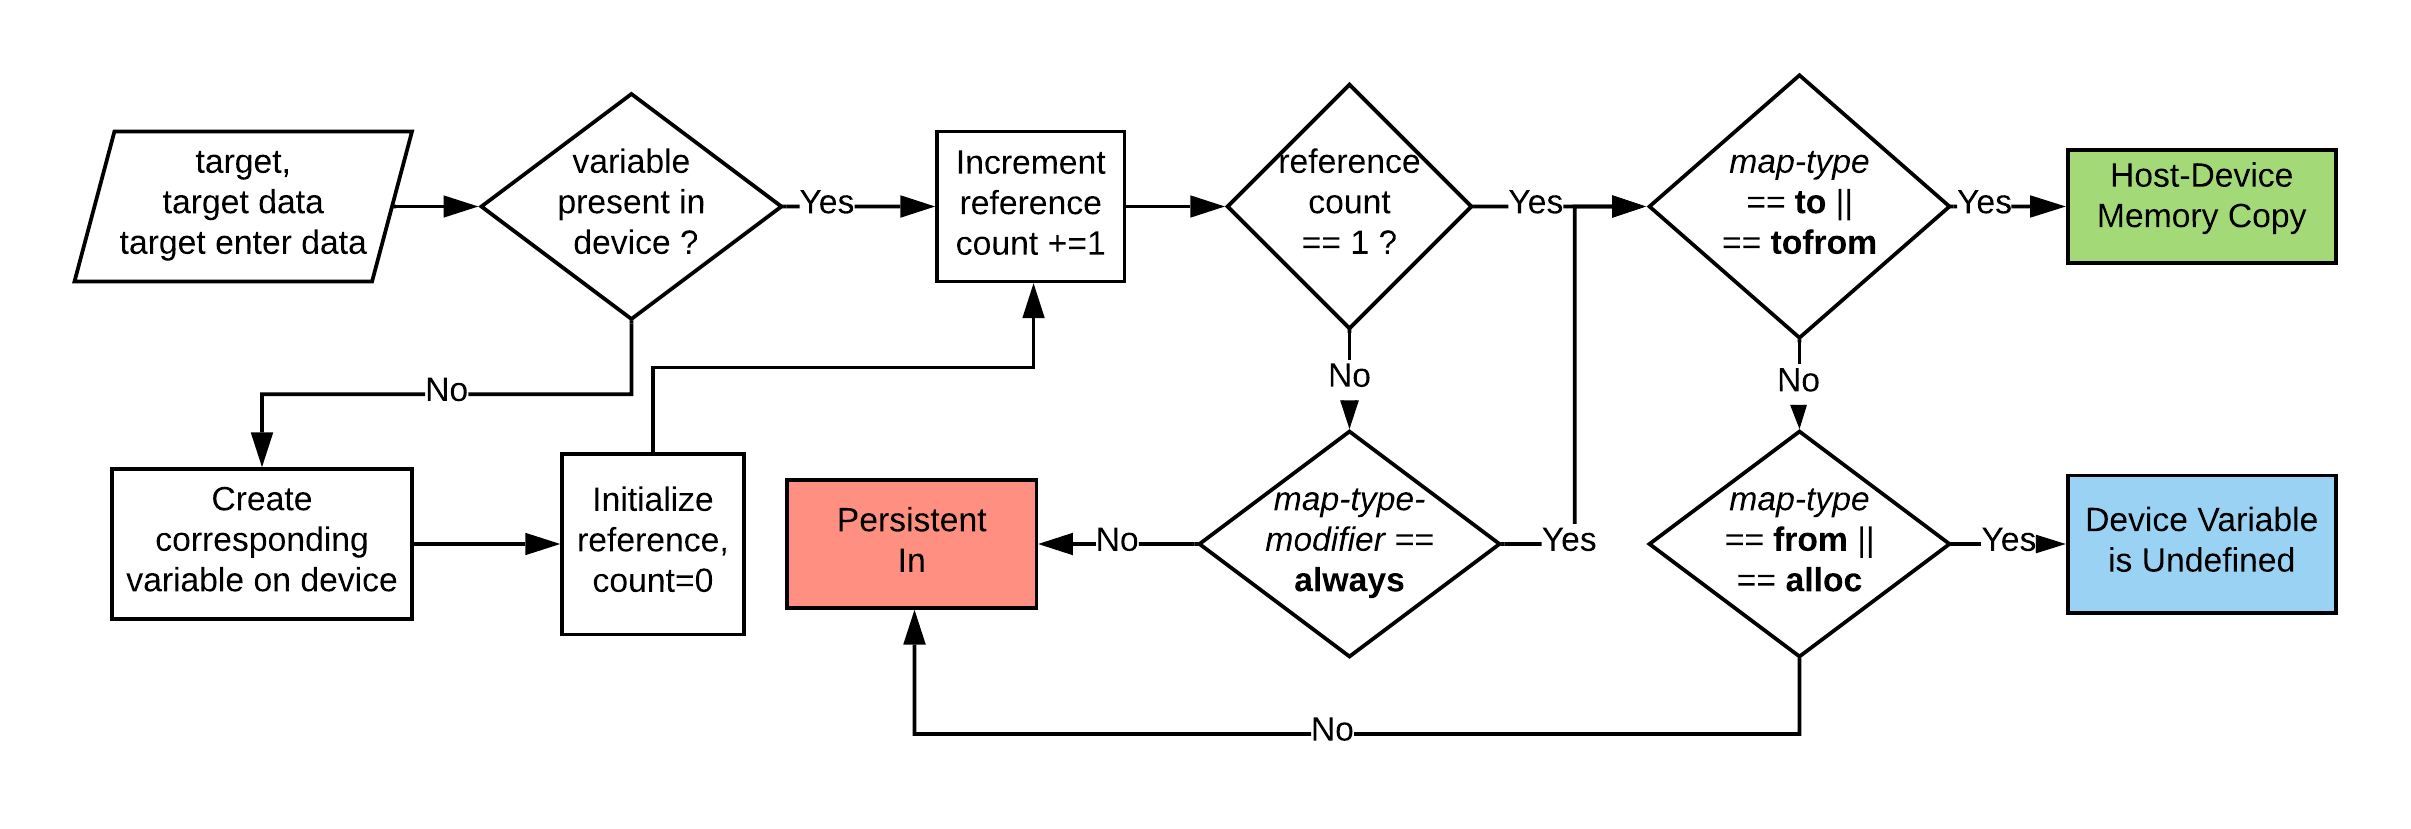
\includegraphics[scale=0.6]{images/data-enter.png}
  \caption{Flowchart for Enter Device Environment}
    \label{host-device-flowchart}    
  \end{subfigure} 
  
%   \hspace{20pt}
  \begin{subfigure}[b]{1\textwidth}
  \centering
    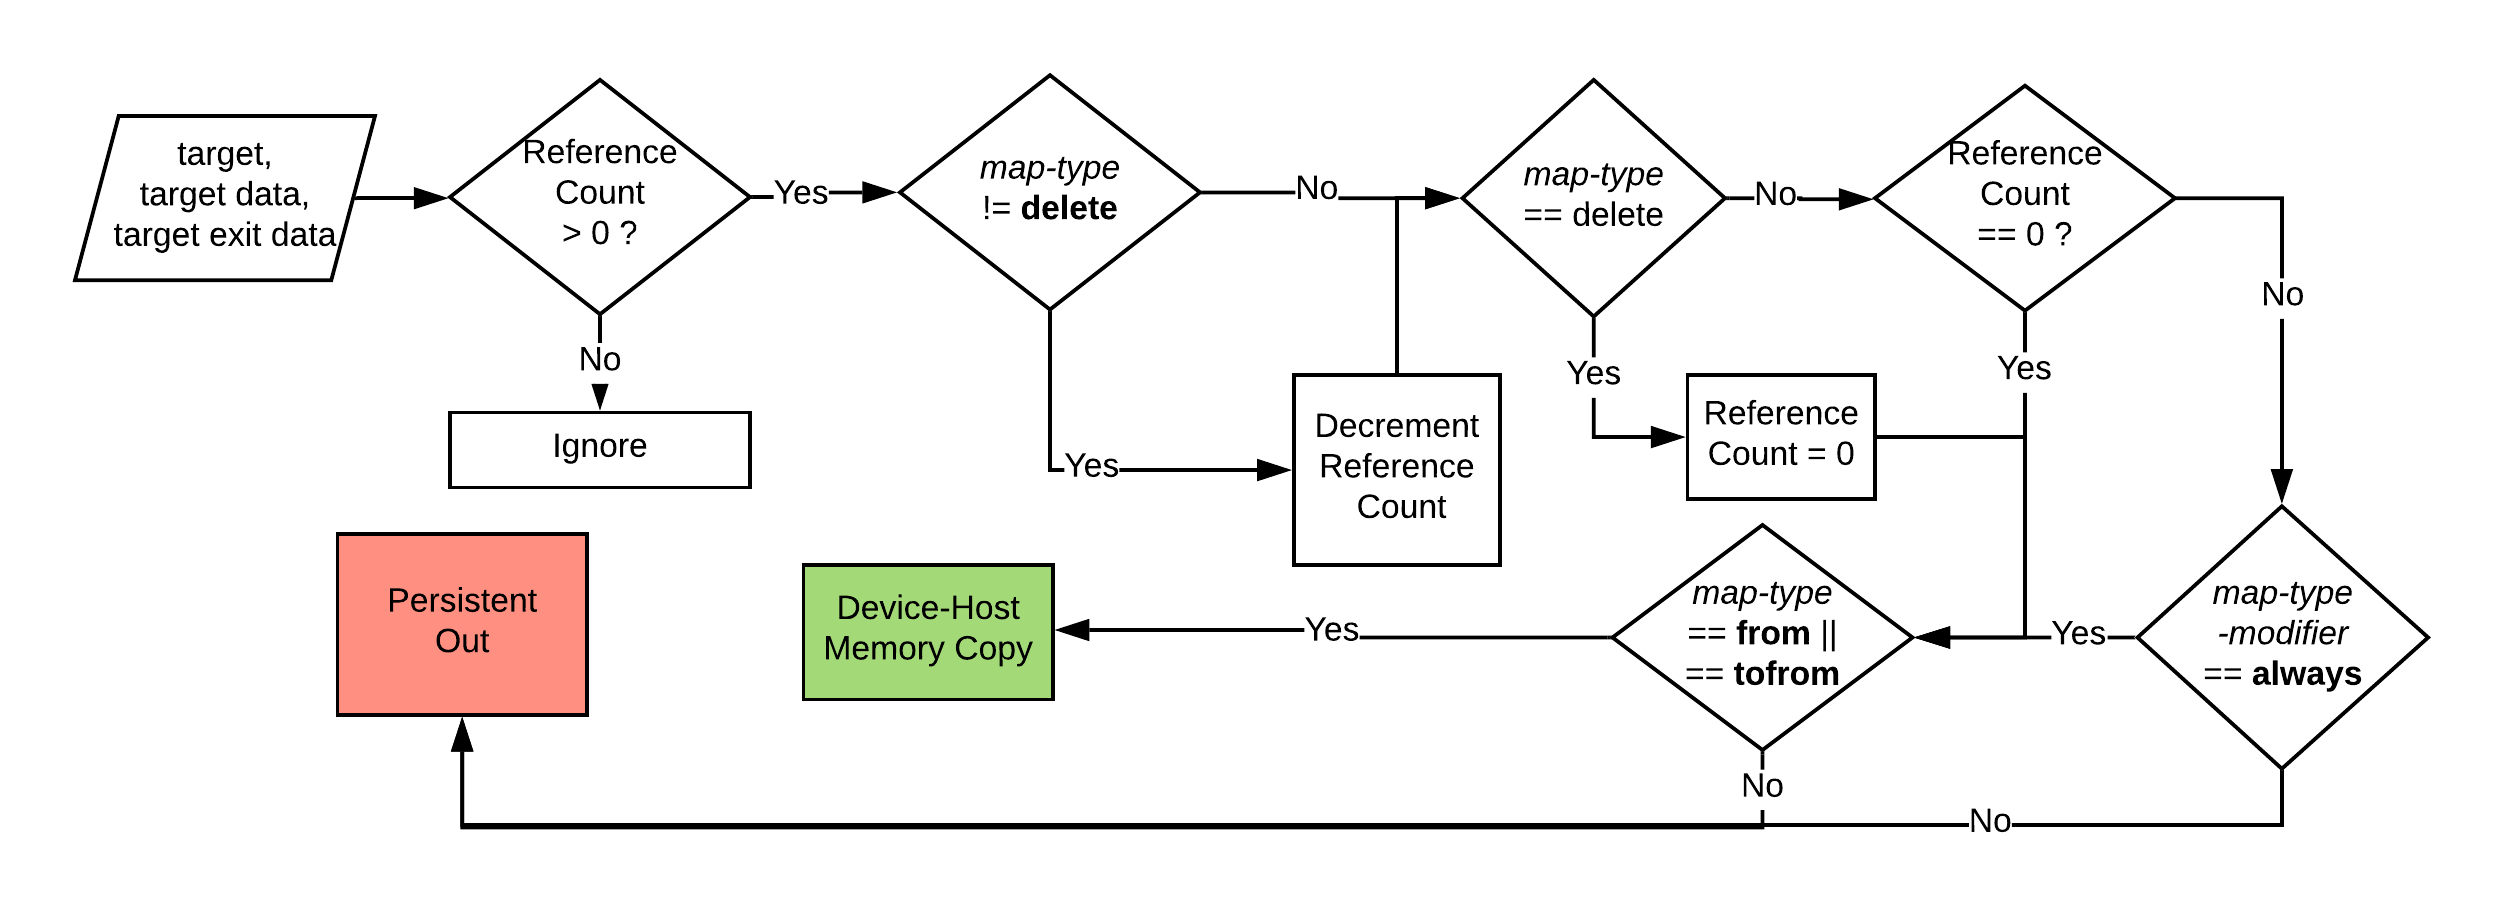
\includegraphics[scale=0.6]{images/data-exit.png}
    \caption{Flowchart for Exit Device Environment}
    \label{device-host-flowchart}    
  \end{subfigure}
  \caption{Flowcharts to show how to interpret the map clause}    
  \label{mapSemantics}
%   \vspace*{-10pt}
\vspace{-20pt}
\end{figure} 
% The OpenMP 4.5 specification specifies the semantics of the \textit{map}
% clause, and \autoref{mapSemantics} illustrates how the spec 
% interprets the data map constructs. 
% The flowchart also motivates our argument that understanding the \textit{map} clause is not trivial, it 
%  shows the complex set of rules defined in the OpenMP 4.5 spec, 
% that is used to determine how to map a  host variable to the corresponding list item in the device data environment.
% We make a simplifying assumption that the CPU host is the current 
% task's data environment and the device is a GPU, and hence the mapping from the host to the device
% refers to the Device-Host and Host-device memory copy.
As \autoref{mapSemantics} shows, OpenMP 4.5 specification uses the reference count of a variable, to decide when to introduce 
a device/host memory copy. The host to device memory copy is 
introduced only when the reference count is incremented from 0 to 1 and the ``to'' attribute is present. 
Then the reference count is incremented every time a 
new device map environment is created. 
The reference count is decremented on encountering a ``from'' or ``release'' 
attribute, while exiting the data environment. 
Finally, when the reference count is decremented to zero from 1, and the 
``from'' attribute is present, 
the variable is mapped back to the host from the device.
% \autoref{statemachine} shows an example state machine, 
% to decide when to insert the memory copies.
% \begin{figure}
% %  \hspace*{-30pt}
%     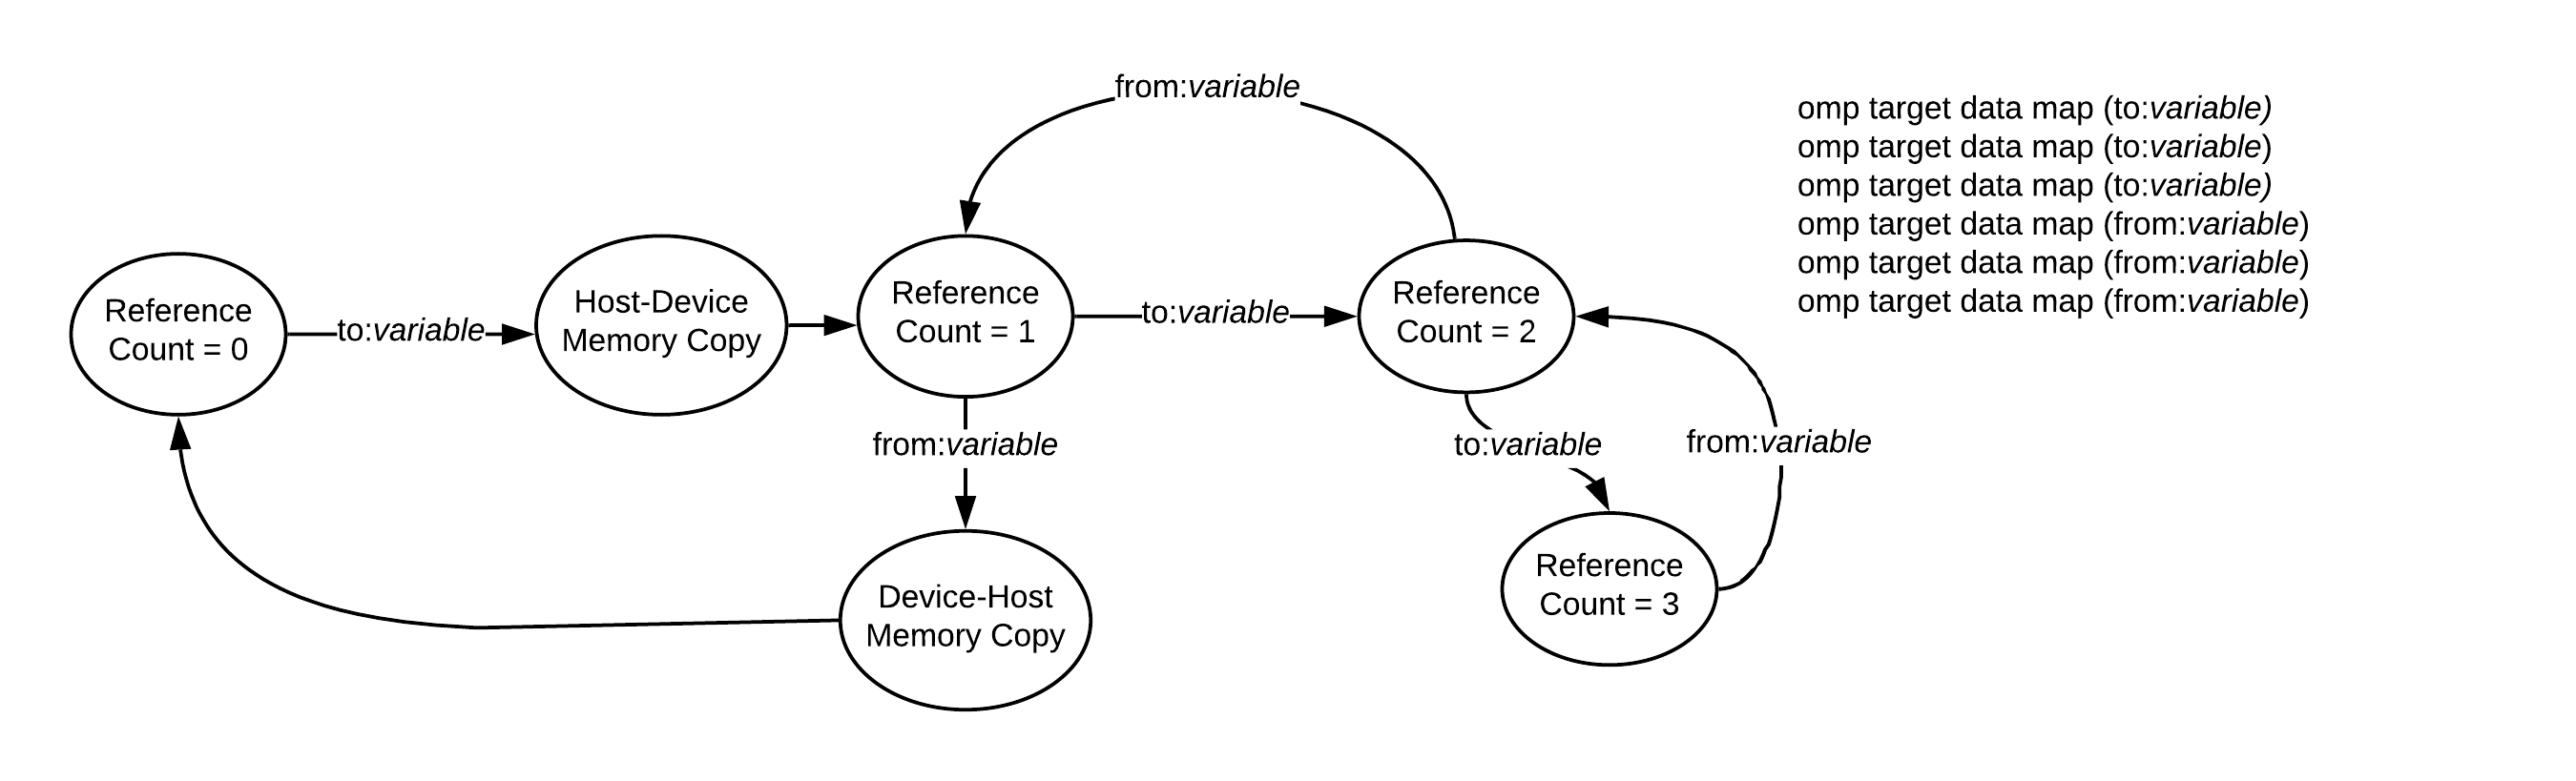
\includegraphics[scale=0.6]{images/statemachine.png}
%     \caption{State Machine for inserting Host/Device Memory Copies } \label{statemachine}
% \end{figure}
\vspace{-10pt}
\subsection{Our Solution}
% \vspace{-50pt}
To address the complexity of using OpenMP's target map 
clauses, we propose a static analysis 
tool called OmpSan to perform OpenMP code ``sanitization''.
OmpSan is a compile-time tool, which does static verification 
of data mapping constructs based on a dataflow analysis.
The key principle guiding our approach is that, ``An OpenMP program is expected to yield the same result when enabling
or disabling OpenMP constructs''.
% this issue as first-aid error detection, we propose a
% compile-time approach based on dataflow analysis. 
% The key principle guiding our error detection approach is that
% ``A user program yields the same result when enabling or disabling
% OpenMP constructs''.
% \footnote{With the exception of privatization clauses, which is unrelated to our goal, and beyond the scope of this work}.
Our approach detects errors by comparing 
dataflow information (reaching definitions via
LLVM's memory SSA representation \cite{llvm-memoryssa-url}) 
between the OpenMP and baseline code.  We developed an
LLVM-based implementation of our approach and evaluated its
effectiveness using several case studies.
Our major contributions include the fo1llowing.
\begin{itemize}
\vspace{-3pt}
\item An algorithm to analyze OpenMP runtime library calls inserted by Clang in the LLVM IR, to infer the host/device memory copies. We expect 
that this algorithm will have applications beyond our OmpSan tool. 
% according to OpenMP 4.5 semantics
\item A static analysis technique to validate if the host/device memory copies respect the original memory def-use relations. 
% \item Reporting error/warnings on usage of data mapping constructs 
% on given user programs
\item Diagnostic information to understand how the map clause affects the 
host and device data environment. 
\end{itemize}\vspace{-10pt}
The paper is organized as follows. 
\autoref{s2} provides certain motivating examples, 
that show common issues  and difficulties in usage of 
OpenMP's \textit{data map} construct. 
\autoref{s03} provides the background information 
that we use in our analysis.
\autoref{s3} presents an overview of our approach to validate 
the usage of data mapping constructs. 
\autoref{s4} presents the LLVM implementation details, and 
\autoref{s5} presents the evaluation and some case studies. 
\autoref{limitation} also lists some of the limitations of 
our tool, some of them common to any static analysis.  
% According to the OpenMP 4.5 semantics, the \texttt{target}, 
% \texttt{target data}, and the \texttt{target enter data} 
% constructs maps host variables to a device data environment. Essentially 
% for the GPU, it inserts host-device and device-host memory copies. 
% The \texttt{map} clause is used to specify how a variable is mapped 
% from the host to the device environment.


\section{Motivating Examples}
\label{s2}
% \vspace{-10pt}
To motivate the utility and applicability of OMPSan,
we discuss three potential errors in user code arising from 
improper usage of the data mapping constructs.
% We discuss potential errors in the user code arising 
% from improper usage of the data mapping constructs, 
% and illustrate how easy it is to incorrectly use the map 
% construct. 
% The accompanying examples motivate the utility and applicability of our proposed analysis and the tool OMPSan.

% We show several common pitfalls of the OpenMP data map construct, 
% and illustrate how easy it is to incorrectly use the map 
% construct, and thus motivate the need for our tool.
\vspace{-10pt} 
\subsection{Default Scalar Mapping}
\subsubsection{Example 1:}
Consider the snippet of code in \autoref{incorrectegs1}.
Note that the definition of \textsf{sum} on line 5 does not reach line 6,
since the variable \textsf{sum} is not mapped explicitly using the \texttt{map} 
clause. As such, \textsf{sum}  is implicitly \texttt{firstprivate}. 
As \autoref{incorrectegs-fix1} shows, an explicit \texttt{map} clause with the
\texttt{tofrom} attribute is essential to specify the copy in and copy out of
 \textsf{sum} from device.

\begin{minipage}{.4\textwidth}
\begin{lstlisting}[style=customc, frame=tlrb, caption={Default scalar map}, label=incorrectegs1]
int A[N], sum=0, i;
#pragma omp target
#pragma omp teams distribute parallel for reduction(+:sum) {
    for(i=0; i<N; i++) {
      sum += A[i];
    }
  }  
  printf("\n%d",sum);
\end{lstlisting}
\end{minipage}\hfil
\begin{minipage}{.4\textwidth}
\begin{lstlisting}[style=customc, frame=tlrb, caption={Explicit map}, label=incorrectegs-fix1]
int A[N], sum=0;
#pragma omp target map(tofrom:sum)
#pragma omp teams distribute parallel for reduction(+:sum) {
    for( int i=0; i<N; i++) {
      sum += A[i];
    }
  }
  printf("\n%d",sum);
\end{lstlisting}
\end{minipage}
\vspace{-10pt}
\subsection{Reference Count Issues in OpenMP 4.5}
% \subsubsection{Example 2:}
% \autoref{incorrectegs3} shows an example of data-mapping 
% attributes across different data environments.
% The array \textsf{B} is specified as \texttt{alloc} in the first 
% data environment. As per OpenMP 4.5 semantics (\autoref{mapSemantics}), when 
% exiting a data environment where a variable is mapped as \texttt{alloc},  there is no need to decrement the reference count.
% We can track the reference count for \textsf{B} is as follows, 
% \begin{itemize}
% \vspace*{-8pt}
%  \item Line 5, reference count = 1
%  \item Line 6, enter data environment, reference count = 2
%  \item Line 8, exit data environment \texttt{alloc}, reference count = 2
%  \item Line 9, exit data environment \texttt{from}, reference count =1
% \end{itemize}
% Note that a variable is mapped back from device to host only if its reference count is decremented to 0 upon exiting the device data environment.
% As such, on Line 12, the value of \textsf{B} is stale, since the updated value from the device  was not mapped back to the host.
% 
% 
% As \autoref{incorrectegs-fix3} shows, replacing \texttt{alloc} 
% with \texttt{from} on line 6, will update the host version of \textsf{B} 
% on exit of the map region at line 9. This is no longer a bug in OpenMP 5.0, since even \texttt{alloc}
%  decrements the reference counter. This example just shows that 
%  certain nuances in the spec can to lead to incorrect behaviour.
% 
% \begin{minipage}{.4\textwidth}
% \begin{lstlisting}[style=customc, frame=tlrb, caption={Usage of alloc}, label=incorrectegs3]
% int A[10], B[10];
% for (int i =0 ; i < 10 ; i++)
%     A[i] = i;
% 
% #pragma omp target enter data map(to:A[0:10]) map(alloc:B[0:10])
% #pragma omp target map(alloc:B[0:10])
% for (int i = 0 ; i < 10; i++)
%     B[i] = A[i];
% #pragma omp target exit data map(from:B[0:10])
% 
% for (int i = 0 ; i < 10; i++)
%     printf("%d",B[i]);
% \end{lstlisting}
% \end{minipage}\hfil
% \begin{minipage}{.4\textwidth}
% \begin{lstlisting}[style=customc, frame=tlrb, caption={Usage of from}, label=incorrectegs-fix3]
% int A[10], B[10];
% for (int i =0 ; i < 10 ; i++)
%     A[i] = i;
% 
% #pragma omp target enter data map(to:A[0:10]) map(alloc:B[0:10])
% #pragma omp target map(from:B[0:10]) 
% for (int i = 0 ; i < 10; i++)
%     B[i] = A[i];
% #pragma omp target exit data map(from:B[0:10])
% 
% for (int i = 0 ; i < 10; i++)
%     printf("%d",B[i]);
% \end{lstlisting}
% \end{minipage}


% 
% 
% can not only 
% error out on such issues, 
% but also the show debug information 
% to help understand how each map construct 
% is interpreted based on its context.
\subsubsection{Example 2:} 
\autoref{incorrectegs2} shows an example of a reference count issue. 
% reference count, user might not get the expected behavior. 
The statement in line 9, which executes on the host, does not read
the updated value of \textsf{A} from the device. 
This is again because of the \texttt{from} clause on line 5, increments 
the reference count to 2 on entry, and back to 1 on exit, hence 
after line 7, \textsf{A} is not copied out to host.
\autoref{incorrectegs-fix2} shows the usage of \texttt{target update} directive 
to force the copy-out and to read the updated value of \textsf{A} on line 11.

This example shows the difficulty in interpreting an 
independent map construct. 
Especially when we are dealing with the global variables 
and map clauses across different functions, 
maybe even in different files, 
it becomes nearly impossible to understand 
and identify potential incorrect usages of 
the map construct. 
Our static analysis tool can report diagnostics and errors with possible fixes to help the developers in using the data mapping clauses.
% incorrect usage of map clause. 
% The user declared the target data environment on line 3, with ``A'' mapped as ``from''. According to the OpenMP 4.5 semantics, the map clause on line 3, 
% will instantiate an uninitialized version of array ``A'' on device, 
% and also associate a reference count with it. The reference count will 
% be set to 1, after the  line 3. Now the map clause on the ``target'' 
% construct, at line 5, will have no affect on the device copy of ``A'', but 
% still it will increment the reference count to 2 at line 5. 
% At the exit of the offloaded loop, after line 7, the reference count 
% is 2, hence the ``from'' clause on line 5 will not have any affect, 
% other than decrementing the reference count to 1. 
% Now the line 9, that is executed on the host, will not 
% be reading the updated version of ``A'' from the device, line 7, 
% because ``A'' was not mapped back to the host after line 7.
% On exit of the data map region at line 10, the reference count is 
% decremented to 0, and only then the device copy of ``A'' is 
% mapped back and copied to the host. This is because of the 
% ``from'' map attribute on line 3. In this example, ``from'' 
% attribute on line 5, has no affect. 
% To fix this issue, we need to use the update clause as shown in 
% \autoref{incorrectegs-fix2}.

\begin{minipage}{.37\textwidth}
\begin{lstlisting}[style=customc, frame=tlrb,  caption={Reference Count}, label=incorrectegs2]
#define N 100                                                                                            
int A[N], sum=0;
#pragma omp target data map(from:A[0:N]) 
  {
    #pragma omp target map(from:A[0:N]) {
      for(int i=0; i<N; i++) {
        A[i]=i;
      }
    }
    for(int i=0; i<N; i++) {
      sum += A[i];
    }
  }
\end{lstlisting}
\end{minipage}\hfil
\begin{minipage}{.45\textwidth}
\begin{lstlisting}[style=customc, frame=tlrb, caption={Update Clause}, label=incorrectegs-fix2]

#define N 100                                                                                            
int A[N], sum=0;
#pragma omp target data map(from:A[0:N]) 
  {
    #pragma omp target map(from:A[0:N]) {
      for(int i=0; i<N; i++) {    
        A[i]=i;
      }
    }
    #pragma omp target update from(A[0:N])  {
      for(int i=0; i<N; i++) {
        sum += A[i];
      }
    }
  }
\end{lstlisting}
\end{minipage}

% In the next section, we will introduce our static analysis tool, 
% which can identify such issues with the incorrect/unexpected 
% usage of OpenMP data mapping constructs. 
% Assuming the correct/expected
% behavior is same as when executing the OpenMP program by ignoring all the 
% OpenMP constructs.
% Lets look at an example to motivate that determining when to insert the
% memory copies is non-trivial and can result in incorrect programs, 
% if the programmer does not understand the OpenMP spec precisely. 
% \autoref{datamapping1} shows an example of incorrect usage of the openmp data mapping clause. 
% On line 4, the map clause, specifies \textit{tofrom}, hence at the entry and 
% exit of the omp region, host-device and device-host memory copy is introduced. 
% That is, a new device copy for the variable $sum$ is made at line   4, and 
% the host $sum$ is copied to the device $sum$. Line 6, increments the value to 1. 
% Line 7, where the region ends, copies back the device $sum$ to host $sum$, and hence
% line 8 prints the correct value of $sum$. Again Line 9, has the map clause \textit{to}, 
% which copies the host $sum$ to device $sum$ on line 10, but since \textit{from} is missing
% fromt he clause, the host copy is not updated on line 12, since the device to host memory copy
% is not present. Since, the host does not access, $sum$ on line 13, this is a valid behaviour. 
% But again on line 14, \textit{tofrom} maptype is used, but this time, since the $sum$ 
% was already present on the device, a host device memory copy is not inserted. Also, 
% since the reference count for $sum$ on device is now 2, and the \textit{from} maptype 
% only decrements the reference count to 1, the device-host copy is also not inserted on line 17. 
% This is a common mistake user can make, if he does not carefully follow the OpenMP 4.5 specs.
% 
% \begin{lstlisting}[style=customc, caption={data map clause}, label=datamapping1]
% int main()
% {
%     int sum = 0 ;
%     #pragma omp target data map (tofrom:sum)
%     {  /*H->D*/
%         sum++;  /* sum = 1 */
%     } /*D->H*/
%     printf("%d",sum); /* 1 */
%     #pragma omp target data map (to:sum)  
%     {  /*H->D*/
%         sum++;  /* sum = 2 */
%     }    
%     /* printf("%d",sum);  1 */
%     #pragma omp target data map (tofrom:sum) 
%     {
%         sum++;  /* sum = 3 */  
%     } 
%     printf("%d",sum); /* 3 */
%     return 0;
% }
% \end{lstlisting}


% \begin{lstlisting}[style=customc, caption={data map clause}, label=datamapping1]
%  static void init_ui(int d1, int d2, int d3)
% {
%   int i, j, k;
% 
% #pragma omp target map (alloc: u0_real,u0_imag,u1_real,u1_imag,twiddle)                                                                                                                                            
% //#pragma omp target update to(u0_real,u0_imag,u1_real,u1_imag,twiddle)
%   {
% //#pragma omp target 
% #pragma omp teams distribute 
%     for (k = 0; k < d3; k++) {
% #pragma omp parallel for 
%       for (j = 0; j < d2; j++) {
%         for (i = 0; i < d1; i++) {
%           u0_real[k*d2*(d1+1) + j*(d1+1) + i] = 0.0; 
%           u0_imag[k*d2*(d1+1) + j*(d1+1) + i] = 0.0; 
%           u1_real[k*d2*(d1+1) + j*(d1+1) + i] = 0.0; 
%           u1_imag[k*d2*(d1+1) + j*(d1+1) + i] = 0.0; 
%           twiddle[k*d2*(d1+1) + j*(d1+1) + i] = 0.0; 
%         }
%       }    
%     }    
%   }
% }
% static void evolve(int d1, int d2, int d3)
% {
%   int i, j, k;
% #pragma omp target map (alloc: u0_real,u0_imag,u1_real,u1_imag,twiddle)
%   {
% #pragma omp teams distribute
%     for (k = 0; k < d3; k++) {
% #pragma omp parallel for
%       for (j = 0; j < d2; j++) {
% #pragma omp simd
%         for (i = 0; i < d1; i++) {
%           u0_real[k*d2*(d1+1) + j*(d1+1) + i] = u0_real[k*d2*(d1+1) + j*(d1+1) + i]*twiddle[k*d2*(d1+1) + j*(d1+1) + i];
%           u0_imag[k*d2*(d1+1) + j*(d1+1) + i] = u0_imag[k*d2*(d1+1) + j*(d1+1) + i] *twiddle[k*d2*(d1+1) + j*(d1+1) + i];
%           u1_real[k*d2*(d1+1) + j*(d1+1) + i] = u0_real[k*d2*(d1+1) + j*(d1+1) + i];
%           u1_imag[k*d2*(d1+1) + j*(d1+1) + i] = u0_imag[k*d2*(d1+1) + j*(d1+1) + i];
%         }
%       }
%     }
%   }
% }
% ft.c:#pragma omp target map (alloc: u0_real,u0_imag,u1_real,u1_imag,twiddle)
% ft.c:#pragma omp target map (alloc: u0_real,u0_imag,u1_real,u1_imag,twiddle)
% ft.c:#pragma omp target map(alloc:twiddle)
% ft.c:#pragma omp target map(alloc: u_real,u_imag) 
% ft.c:#pragma omp target map(alloc: u_real,u_imag) map(to:t)
% ft.c:#pragma omp target map(alloc: gty1_real,gty1_imag,gty2_real,gty2_imag, u1_real, u1_imag)\
% ft.c:#pragma omp target map ( alloc: u1_real, u1_imag, u_real,u_imag)\
% ft.c://#pragma omp target map(alloc: gty1_real,gty1_imag,gty2_real,gty2_imag,\
% ft.c://#pragma omp target map(alloc: gty1_real,gty1_imag,gty2_real,gty2_imag,\
% ft.c:#pragma omp target map (alloc: u1_real, u1_imag, u_real,u_imag, gty1_real, gty1_imag, gty2_real, gty2_imag) 
% ft.c://#pragma omp target map(alloc: gty1_real,gty1_imag,gty2_real,gty2_imag,\
% ft.c:#pragma omp target map (alloc: u1_real, u1_imag, u_real,u_imag, gty1_real, gty1_imag, gty2_real, gty2_imag) 
% ft.c:#pragma omp target map (alloc: u1_real, u1_imag) map(tofrom: temp1, temp2)
% \end{lstlisting}

\section{Background}
\label{s03}
\subsection{Memory SSA form} Our analysis is based on the LLVM 
 Memory SSA \cite{llvm-memoryssa-url} \cite{Novillo_memoryssa}, 
 which is an imprecise 
implementation of Array SSA\cite{Knobe:1998:ASF:268946.268956}.
The Memory SSA is a virtual IR, that captures the def-use 
information for array variables. Every definition is 
identified by a unique name/number, which is then referenced 
by the corresponding use.
% Memory SSA captures the 
% use-def chains for every memory access in the program. 
% We construct the def-use chains for each array variable, 
% based on the Memory SSA. 
% The store instruction 
% corresponds to the definition, and load instruction corresponds 
% to memory use, and Memory Phi nodes merge the \textit{may} reach 
% definitions. 
% LLVM Memory SSA is a virtual IR, where every definition and phi 
% node creates a new version of memory, which are numbered.

The Memory SSA IR has the following kinds of instructions/nodes, 
\begin{itemize}
% \vspace{-10pt}
 \item $INIT$, a special node to signify uninitialized or live on 
 entry definitions
 \item $N' = MemoryDef(N)$, $N'$ is an operation which may modify memory, 
 and $N$ identifies the last write that $N'$  clobbers.
 \item $MemoryUse(N)$, is an operation that uses the memory written 
 by the definition $N$, and does not modify the memory. 
 \item $MemPhi(N_1,N_2,...)$, is an operation corresponding to a
 basic block, and $N_i$ is one of the may reaching definitions, 
 that could flow into the basic block.
\end{itemize}

We make the following simplifying assumptions, to keep the analysis
tractable
\begin{itemize}
% \vspace{-8pt}
 \item Given an array variable we can find all the  corresponding
 load and store instructions. So, we cannot handle cases, when pointer
 analysis fails to disambiguate the memory a pointer refers to.
 \item A $MemoryDef$ node clobbers the array associated 
 with its store instruction. As a result, write to any array location, 
 is considered to update the entire array.
 \item $MemoryPhi$ nodes are inserted only at the entry 
 of basic blocks, which have more than one $MemoryDef$s that can 
 flow into the basic block.
 \item We analyze only the array variables that 
 are mapped to a target region. 
\end{itemize}

% \vspace{-16pt}
\subsection{Scalar Evolution Analysis}\vspace{-5pt}
LLVM's Scalar Evolution (SCEV) is a very powerful technique
that can be used to analyze the change in 
the value of scalar variables over iterations of a loop, as a chain 
of recurences. 
We can use the SCEV analysis to represent the loop induction variables 
as chain of recurrences. 
This mathematical representation 
can then be used to analyze the variables used to index into memory 
operations. 
Then it can be used to symbolically evaluate the 
minimum and maximum value of every array index expression. 
In case the SCEV analysis fails to model an expression, 
we over approximate the range of the array indices to the 
maximum dimensions of the array variable. 
\autoref{s4} has details 
of how we implement the analysis and handle different cases. 

\section{Our Approach}
\label{s3}
% \begin{minipage}{.45\textwidth}
% \begin{lstlisting}[style=customc, frame=tlrb, caption={Example Code 1}, label=memorySSA-example-1]
% 
% L1: for ( i =0 ; i < 100 ; i++) {
%         S1: A[i] = 0;
%     }
% #pragma omp target enter data map(to:A[0:50], alloc:C[0:100])
% #pragma omp target
% L2: for (i=0; i < 100; i++ ) {
%         S2: t = A[i] ;
%         S3 C[i] = t; 
%     }    
% #pragma omp target exit data map( release:C[0:100])
% L3: for (i=0; i < 100; i++) {
%         S4: print(C[i])
%     }
% \end{lstlisting}
% \end{minipage}
% In this work, we assume that variables
% that have corresponding list items across host and device 
% boundary or across different data environment boundaries 
% on the device need to be updated at the edge of such boundaries. 
% Typically this assumption reflects the practical use-case of the variables. 
\vspace{-10pt}
OMPSan assumes certain practical use cases, for example, in \autoref{incorrectegs2}, 
a user would expect the updated 
value of ``A'' on line 11. 
Having said that, a skilled ninja programmer 
may very well expect ``A'' to remain stale, because of their knowledge 
and understanding of the complexities of data mapping rules. 
Our analysis and error/warning reports from this work are 
intended primarily for the former case.

In this section, we outline the key steps of our approach with the algorithm
and show a concrete example 
to illustrate the algorithm in action.
% \vspace{-10pt}
\subsection{Algorithm}
\begin{algorithm}[!htbp]
    \caption{Overview of Data Mapping Analysis}
    \label{dataMapAnalysisAlgo}
    \begin{algorithmic}[1]
        \small 
    \Function{$\textsc{DataMapAnalysis}$}{$Module$}
        \State $MappedArrayVars=\phi$
        \For{$ArrayVar \in MapClauses$}
            \State $MappedArrayVars = MappedArrayVars \cup ArrayVar$
        \EndFor
        \State \texttt{ConstructArraySSA}($Module, MappedArrayVars$)
        \State \texttt{InterpretTargetClauses}($Module, MappedArrayVars$)
        \State \texttt{ValidateDataMap}($MappedArrayVars$)
    \EndFunction
    \Function{$\textsc{ConstructArraySSA}$}{$Module, MappedArrayVars$}
%         \State $MappedArrayVars=\phi$
%         \For{$ArrayVar \in MapClauses$}
%             \State $MappedArrayVars = MappedArrayVars \cup ArrayVar$
%         \EndFor
        \For {$MemoryAccess \in Module$}            
            \State $ArrayVar$ = \texttt{getArrayVar}($MemoryAccess$)
            \If{ 
                $ArrayVar \in MappedArrayVars$ }
            \If { $MemoryAccess  \in OMP\_targetOffload\_Region$}
                \State $targetNode = true$
                \Comment{If Memory Access on device}
            \Else
                \State $targetNode = false$
                \Comment{If Memory Access on host}
            \EndIf
            \State $Range= $ \texttt{SCEVGetMinMax}$(MemoryAccess)$
            \State $underConstruction$= \texttt{GetArraySSA}$(ArrayVar)$
            
            \State \Comment{could be null or incomplete}
            
            \State \texttt{InsertNodeArraySSA}($underConstruction$,$MemoryAccess, targetNode, Range$ )
%             \Comment{Incrementally construct, by adding this access}
            \State  \Comment{Incrementally construct, by adding this access}            
            \EndIf 
        \EndFor
        \EndFunction
        \Function{$\textsc{InterpretTargetClauses}$}{$Module, MappedArrayVars$}
        \For {$ArrayVar \in MappedArrayVars$ }
            \State $ArraySSA =$ \texttt{GetArraySSA}($ArrayVar$)
            \For { \textbf{edge}, $(node, Successornode) \in $ ($ArraySSA$) }
%                 \State $node$ = $edge.from$
                \State $nodeIsTarget =$ \texttt{isTargetOffload}($node$)
                
                \State $succIsTarget =$ \texttt{isTargetOffload}($Successornode$)
                \If { $nodeIsTarget \ != succIsTarget$}
                    \State \texttt{RemoveArraySSAEdge($node$, $Successornode$ )}
                \EndIf                                                
            \EndFor 
        \EndFor 
        \For {$dataMap   \in dataMapClauses$}
            \State $hostNode$ = \texttt{getHostNode}($dataMap$)
            \State $deviceNode$ = \texttt{getDeviceNode}($dataMap$)
            \State $mapType =$ \texttt{getMapClauseType(}$ dataMap$)
                    \State \Comment{alloc/copyIn/copyOut/persistentIn/persistentOut}
                    \State \texttt{InsertDataMapEdge}($hostNode, deviceNode, 
                    mapType$)
        \EndFor
        \EndFunction
        \Function{$\textsc{ValidateDataMap}$}{$MappedArrayVars$}
        \For {$ArrayVar \in MappedArrayVars$ }
            \State $ArraySSA =$ \texttt{GetArraySSA}($ArrayVar$)
            \For { $memUse  \in $ \texttt{getMemoryUseNodes}($ArraySSA$)}
                \State $useRange$ = $\texttt{getReadRange(memUse)}$
                \State $clobberingAccess =$ \texttt{getClobberingAccess}$(ArraySSA, memUse)$
                \If { \texttt{isPartiallyReachable}($ArraySSA, 
                    clobberingAccess, memUse, useRange$) }
                    \State Report WARNING 
%                     \texttt{Report}($ArraySSA, 
%                     clobberingAccess, memUse, useRange$)                
                \ElsIf { \texttt{isNotReachable}($ArraySSA, 
                    clobberingAccess, memUse$) }
                    \State Report ERROR 
%                     \texttt{Report}($ArraySSA, 
%                     clobberingAccess, memUse, useRange$) 
                \EndIf
            \EndFor
        \EndFor    
        \EndFunction
    \end{algorithmic}
\end{algorithm}
\autoref{dataMapAnalysisAlgo} shows an overview 
of our data map analysis algorithm. First, we 
collect all the array variables used in all the 
map clauses in the entire module.
Then line 5, calls the function \texttt{ConstructArraySSA}, 
which constructs the Array SSA for each of the mapped Array variables. 
(In this paper, we use ''Array SSA'' to refer to our extensions to 
LLVM's Memory SSA form by leveraging the capabilities of Array SSA form \cite{Knobe:1998:ASF:268946.268956}.)
Then, we call the function, \texttt{InterpretTargetClauses}, 
which modifies the Array SSA graph, in accordance of the map semantics of the 
program.
Then finally \texttt{ValidateDataMap} checks the 
reachability on the final graph, to validate 
the map clauses, and generates 
a diagnostic report with the warnings and errors.
% inline all user defined functions, and then use 
% the Memory SSA to construct the memory use-def chains, 
% for every array variable. After step 2, we get a graph for each
% memory array, with an edge from a $MemoryDef$
% or $MemPhi$ to the corresponding $MemoryUse$ or $MemPhi$ for the
% reaching definition relation. 
% Then we use the Scalar Evolution Analysis, to compute 
% the range of locations accessed by every memory reference.
% If the analysis fails to compute the range of locations 
% statically, then we over-approximate it to the 
% maximum size of the array.
% 
% Now we interpret
% the semantics of the \texttt{target} construct, 
% to classify the Memory SSA nodes, as executing on host or device.
% Since the device and host have a separate data environment, 
% they refer to different array variables. So in step 5, we remove the edges between host and device nodes. 
% Now according to the semantics of the \texttt{map} clause, 
% the host variables are mapped to the device variables, and 
% vice-versa. At any program point, when a 
% host variable is mapped to device, 
% we find its corresponding reaching definition, 
% and add a special edge from the host $MemoryDef$ or $MemPhi$, 
% to the $MemoryUse$ or $MemPhi$ on the device. 
% Similarly when mapping a device variable to host variable, 
% we add the edge between the corresponding definition on the device
% to the corresponding use on the host.
% In step 6, we also annotate the edges with the array sections 
% according to the \texttt{map} clause.
% 
% Finally, we report an error for every missing use-def 
% edge in our graph, since it indicates a mismatch
% between the sequential use-def relations and the OpenMp 
% reaching definitions. We report a warning, when an edge indicates
% that the array is partially mapped, and the $MemUse$
% could potentially access locations outside the mapped range.

% \begin{algorithm}
%     \caption{Overview of Data Mapping Analysis}
%     \label{dataMapAnalysisAlgo}
%     \begin{algorithmic}[1]
%         \small 
% %         \Function{$\textsc{DataMapAnalysis}$}{$Module$}
%             
%             \State Construct the Memory SSA for each array variable
% %             \State Dataflow analysis on the 
% %             Use Memory SSA to construct the 
% %             use-def graph for each array variable
%             \State Do scalar evolution analysis 
%             to compute the range of each 
%             memory access            
%             \State Interpret the \texttt{omp target} constructs 
%             and mark the nodes in the SSA graphs as host and device
%             \State Remove the edges from the Memory SSA graph which connect         device nodes with host nodes
%             \State Interpret \texttt{map} clauses to insert edges 
%             in the Memory SSA graph, that correspond to 
%             host-device and device-host memory copies, annotated
%             with array sections 
%             \State For every node in Memory SSA graph, 
%             if the edge from reaching definition is missing, 
%             then Report ERROR
%             \State For every edge connecting host, device nodes, 
%             the array section of the edge must be a subset of 
%             the memory access range of the destination node, 
%             else report it as Warning
% % %             \For{$Memory$ $Access  \in \textsc{Memory SSA}$}
% %                 \If{No Edge between Memory Access and reaching definition}	
% %                     \State Error
% %                 \EndIf
% % %             \EndFor    
%         
% %         \EndFunction
%     \end{algorithmic}
% \end{algorithm}
\begin{figure}[h!]
    \centering
    \begin{subfigure}[b]{0.45\textwidth}
        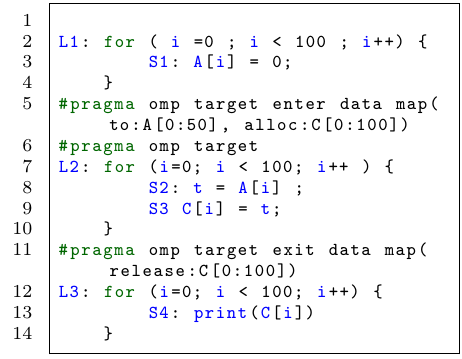
\includegraphics[width=\textwidth]{images/memorySSA-example1.png}
        \caption{Example, user Code}
        \label{fig:memorySSA-example1-s4}
    \end{subfigure}
    ~ %add desired spacing between images, e. g. ~, \quad, \qquad, \hfill etc. 
      %(or a blank line to force the subfigure onto a new line)
    \begin{subfigure}[b]{0.5\textwidth}
        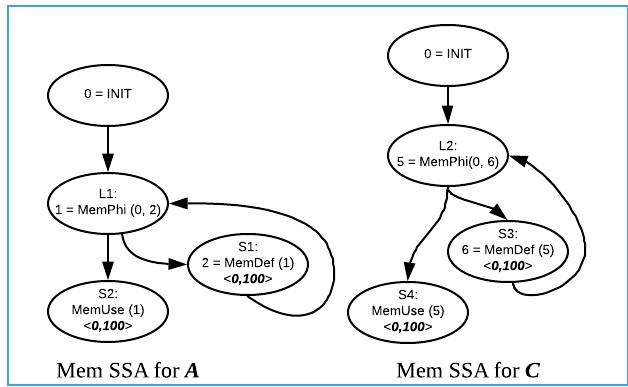
\includegraphics[width=\textwidth]{images/memorySSA-example1-s1.jpg}
        \caption{Memory SSA for sequential version}
        \label{fig:memorySSA-example1-s1}
    \end{subfigure}
    
    ~ %add desired spacing between images, e. g. ~, \quad, \qquad, \hfill etc. 
    %(or a blank line to force the subfigure onto a new line)
    \begin{subfigure}[b]{0.46\textwidth}
        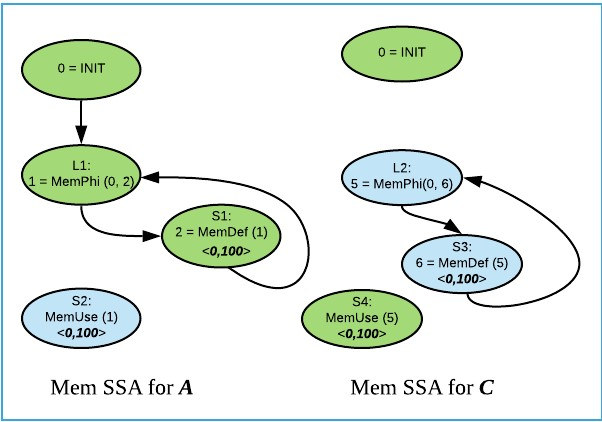
\includegraphics[width=\textwidth]{images/memorySSA-example1-s2.jpg}
        \caption{Classify Host/Device Regions (green=host, blue=device)}
        \label{fig:memorySSA-example1-s2}
    \end{subfigure}
    \begin{subfigure}[b]{0.51\textwidth}
        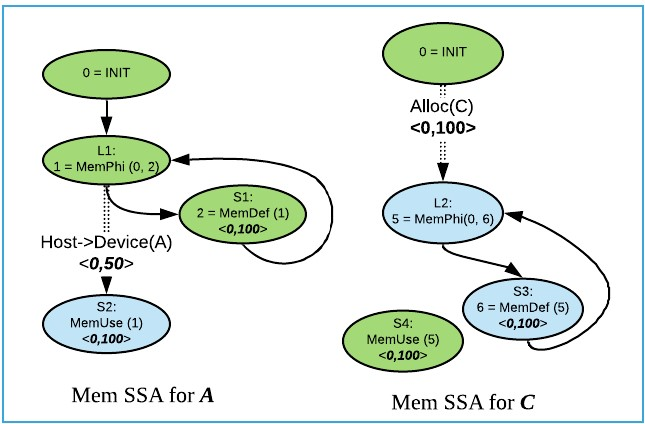
\includegraphics[width=\textwidth]{images/memorySSA-example1-s3.jpg}
        \caption{Host/Device Memory Copies}
        \label{fig:memorySSA-example1-s3}
    \end{subfigure}
    \caption{Example of Data Map Analysis } 
    \label{fig:memorySSA-example1}
%     \vspace{-100pt}
\end{figure}
\vspace{-13pt}
\subsubsection{Example }
Let us consider the first example in \autoref{fig:memorySSA-example1-s4}
to illustrate our approach for analysis of data mapping clauses.
\texttt{ConstructArraySSA} of \autoref{dataMapAnalysisAlgo},  
constructs the memory SSA form for arrays ``A'' and ``C'' as shown in \autoref{fig:memorySSA-example1-s1}.
Then, \texttt{InterpretTargetClauses}, removes 
the edges between host and device nodes, as shown in 
\autoref{fig:memorySSA-example1-s2}, where the host is 
colored green and device is blue.
Finally, the loop at line 29 of the function \texttt{InterpretTargetClauses}, 
introduces the host-device/device-host 
memory copy edges, as shown in 
\autoref{fig:memorySSA-example1-s3}. For example
$L1$ is connected to $S2$
with a host-device memory copy for the enter data map 
pragma with \texttt{to}$:A[0:50]$ on line 5. 
Also, we connect the \textit{INIT} node with $L2$, 
to account for the \texttt{alloc}:$C[0:100]$, which implies 
an uninitialized reaching definition for this example. 

Lastly, \texttt{ValidateDataMap} function, traverses the graph, 
resulting in the following observations:
\begin{itemize}
    \vspace{-5pt}
 \item (Error) Node $S4$:$MemUse(5)$ is not reachable from its 
corresponding  
 definition  $L2:5 = MemPhi(0,6)$ 
 \item (Warning) Only the partial artial array section $A[0:50]$, is reachable from definition
 $L1: 1 = MemPhi(0,2)$ to $S2:MemUse(1)\langle 0:100 \rangle $
\end{itemize}
% These conclusions from our analysis
% are reported to the user along with line numbers from the program, 
\autoref{s5} contains other examples of the errors and warnings 
discovered by our tool. 
\vspace{-15pt}
% 
% 
% % TODO: Delete following lines 
% verify the correctness of the \textit{map} clauses used by a programmer. 
% \autoref{fig:memorySSA-example1-s4} shows a small program fragment, to illustrate the usage of map clause. \autoref{fig:memorySSA-example1-s1}  shows the memory SSA 
% constructed from the program. We can see the use-def chains for the two memory variables $A$ and $C$ individually. The memory SSA clearly shows the uses and the reaching definitions for the corresponding memory variable. 
% The next step is to interpret the target offload constructs used in the program. 
% The target construct is used to offload a region of code onto a device. \autoref{fig:memorySSA-example1-s2} shows the interpretation of the target construct at line 6 of the program.  
%  The figure uses a color code, 
% to illustrate that the red statements are in the device environment, while the green nodes are the host data environment. 
% In this step, we also remove the memory use-def edges that are across two different environments. So for example, there is no edge between 
% L1 and S2, since the L1 loop is executed on the host, while the S2 is on the device. 
% The last step of our analysis is to interpret the \textit{map} clause used in the program, and add special edges in the memory SSA graph, that corresponds to the host/device memory copy. This step follows the algorithm depicted in \autoref{mapSemantics}. So because of the to map clause on line 5, there is an edge between L1 and S2, which respects the reaching definitions for S2 as per \autoref{fig:memorySSA-example1-s1}. 
% Also, the Alloc edge from init node to L2, signifies the alloc map clause for memory variable $C$.  
% Now, for every Memory Use node, we can validate if there is an edge from its corresponding memory def.
% Otherwise, the \textit{map} clauses were used incorrectly in the user program. 
% So for example, there is still a missing edge between Memory use at statement S4. This means map clauses are wrong and S4 is not reading the appropriate value. 
% \subsubsection{Example 2} 
% For our next example, We modify the \autoref{fig:memorySSA-example1-s4}, with the following map clauses, 
% \begin{verbatim}
%  #pragma omp target enter data map(to:A[0:50], alloc:C[0:100])
%  #pragma omp target exit data map(from:C[0:100])
% \end{verbatim} 
% \autoref{memorySSA-3} shows the SSA graphs 
% for the array ``A'' and ``C''
%  and the final graph after interpreting the map clauses. 
% We report the following warning, after our analysis,
% \begin{itemize}
%  \item Warning, Node $S2$:$MemUse(1)$ uses, $<0,100>$, 
%  which is not a subset of $<0,50>$
% \end{itemize}
% \begin{figure}
% % \hspace*{-80pt}
% 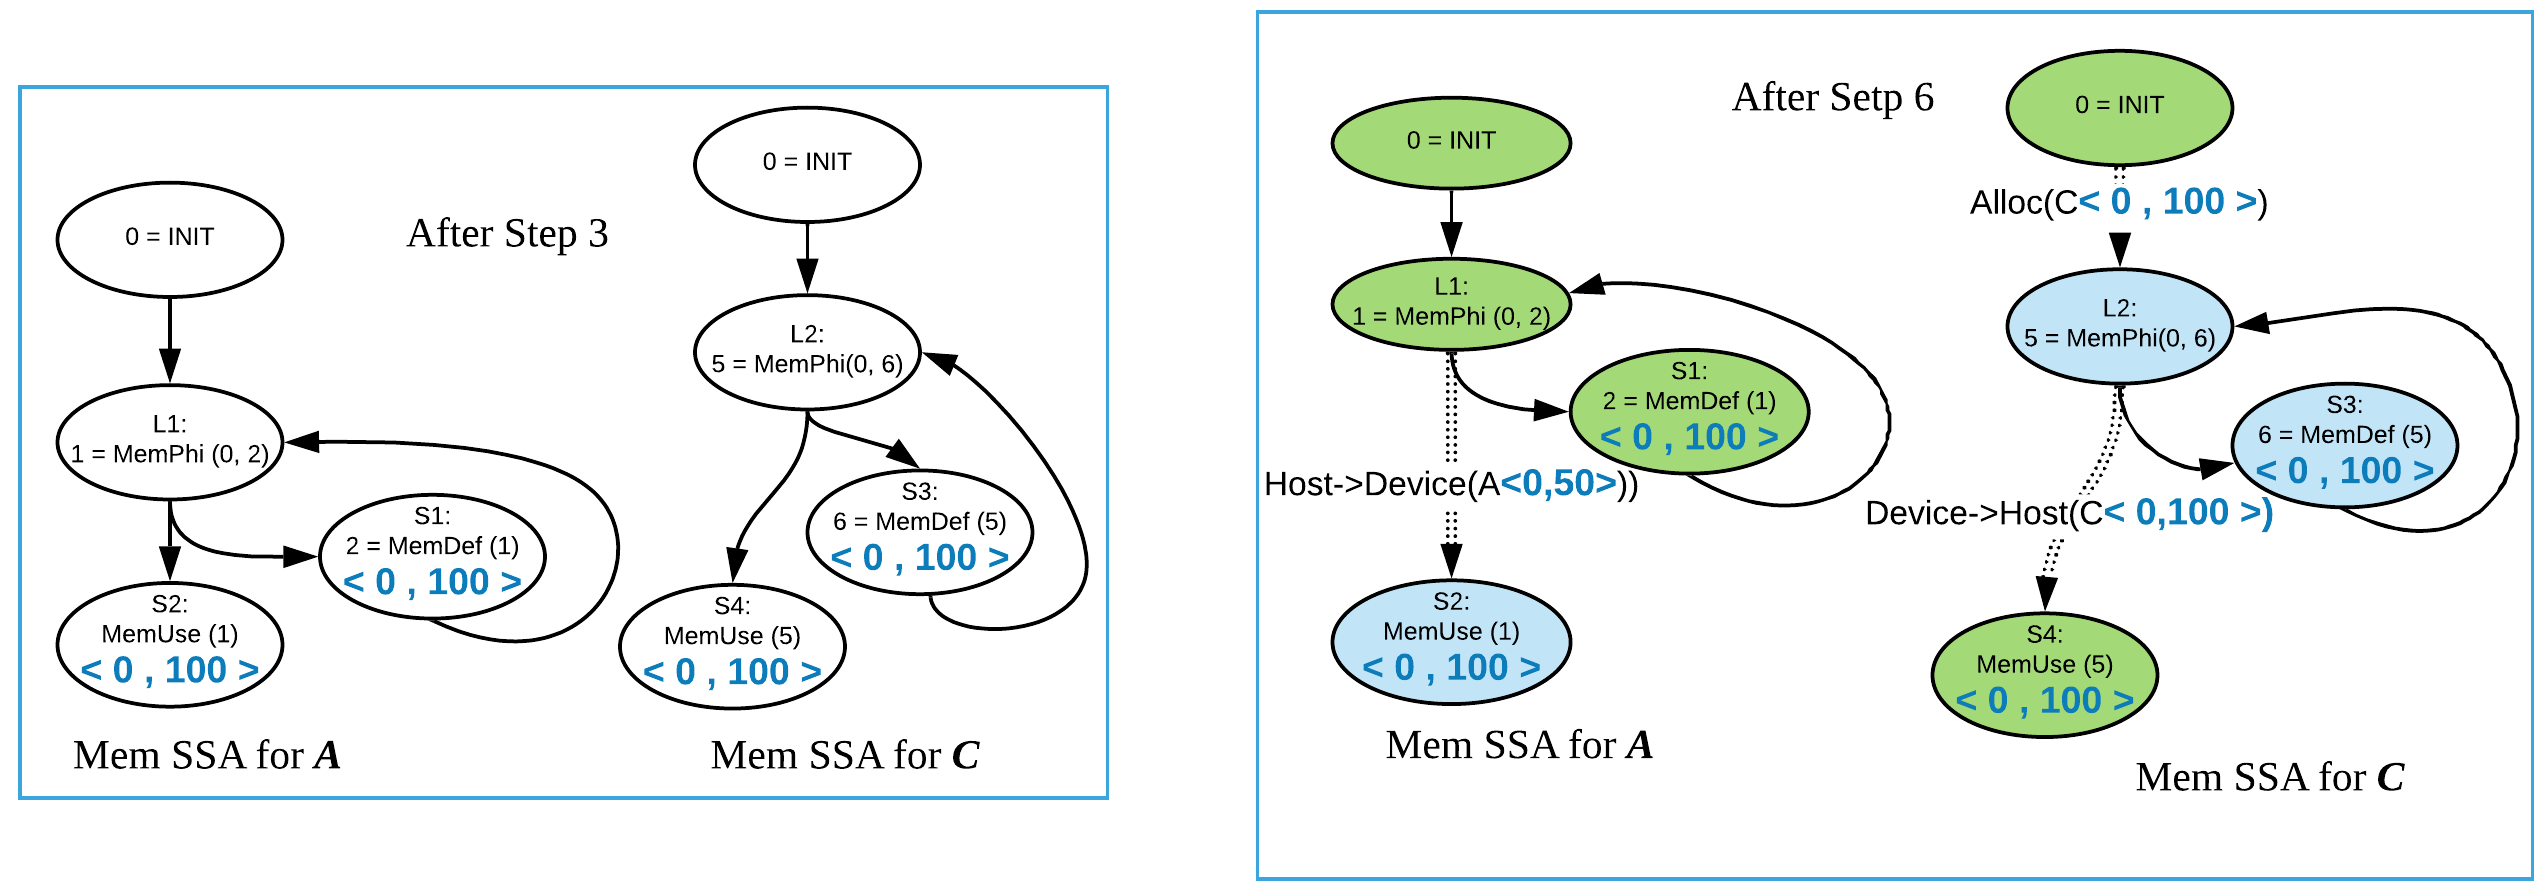
\includegraphics[scale=0.17]{images/memorySSA-3.png}
% \caption{Data Map Analysis Example 2} \label{memorySSA-3}
% \end{figure}
% \subsection{Array Sections}
% \label{SEC:array-sec}
% Next, we look at how to validate the array sections used in the map clause.
% 
% We start with the memory SSA graphs for each memory variable. Each memory def and Memory use corresponds to a statement in the user program. We can analyze the corresponding statement to figure out the index expressions, and the range of values that the expression evaluates to, as shown in \autoref{memorySSA-3}. For example, the index expression at statement S1, has a minimum value of 0 and a maximum value of 100. If the range of the index expression cannot be evaluated statically, then we approximate the range to the size of the memory variable. The size of an array variable is known statically, and the size of dynamically allocated memory variables can be obtained by parsing the corresponding malloc instruction.
% With these annotations, in place, we have a conservative estimate of the range of locations that each memory access refers to. Next step is to interpret the array sections used in the map clauses by the user. It is possible only if the user used compile time constants to specify the array sections in the map clause, as shown in \autoref{memorySSA-3}.
% Each edge between two nodes of different data environments is now annotated with a range. For each such edge, we validate that the corresponding use range is a subset of the range of the edge. Since this analysis is an overapproximation, the violation of this property need not always be an error. Hence we classify this property as a warning.
% \begin{figure}
% \hspace*{-60pt}
% 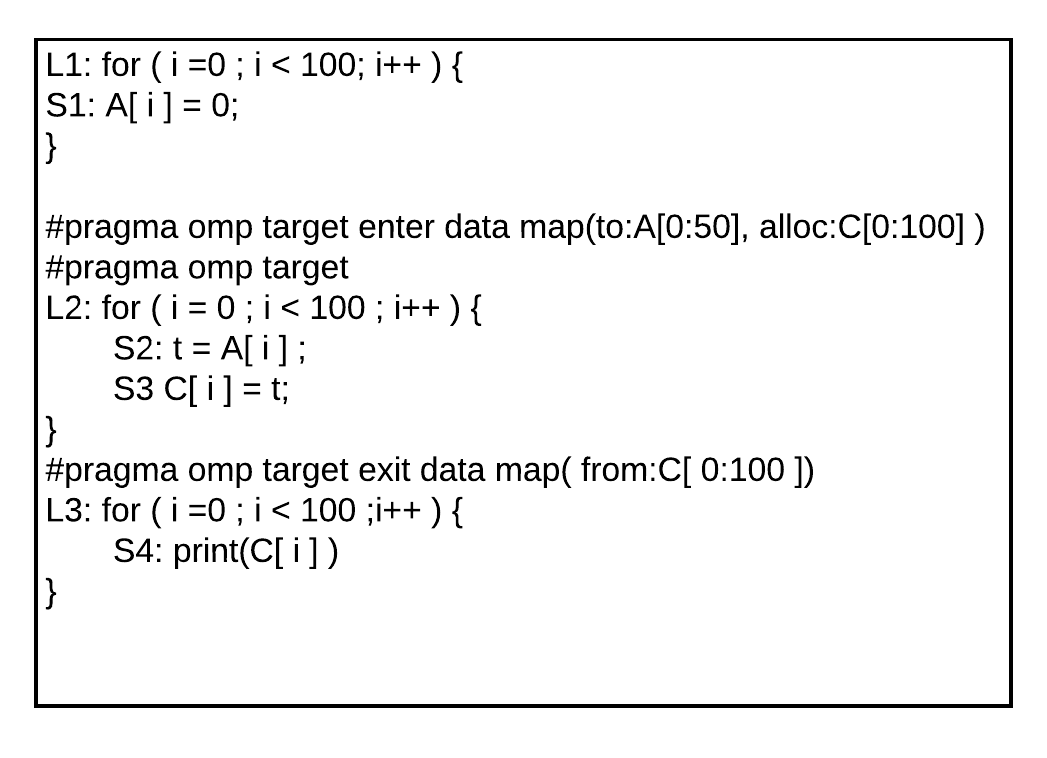
\includegraphics[scale=0.3]{images/memorySSA-3-egs.png}
% \caption{The Algorithm to determine when to insert host-device memory copy} \label{memorySSA-3-egs}
% \end{figure}


\section{Implementation}
\label{s4}
% \vspace{-10pt}
We implemented our framework in LLVM (forked from commit $360853$ on May 15 2019).
In LLVM the OpenMP constructs are lowered to runtime calls in Clang, so 
in the LLVM IR we only see calls to the OpenMP runtime. 
There are several limitations of this approach with respect 
to high level analysis like the one OMPSan is trying to accomplish.
%disadvantages of this approach especially with respect to our analysis. 
For example, the region of code that needs to be offloaded to a device 
is opaque since it is moved to a separate function. 
These functions are in turn called from the OpenMP runtime library. 
As a result, it is challenging to perform a global data flow analysis 
for the memory def-use information of the offloaded region. 
To simplify the analysis, we have to compile with clang twice. 

First, we compile the OpenMP program with the flag that enables
parsing the OpenMP constructs, and compile it again without the flag, 
so that Clang ignores the OpenMP constructs and instead generates the 
baseline LLVM IR for the sequential version. 
During the OpenMP compilation pass, we execute 
our analysis pass, which parses the runtime library calls 
and generates a csv file that records all the user specified 
``target map'' clauses, as explained in \autoref{interpreting-openmp-pragmas}.

Next we compile the program by ignoring the OpenMP pragmas, 
and perform  whole program context and flow sensitive data flow analysis
on LLVM code generated from the sequential version, to construct
the Memory def-use chains, explained in 
\autoref{baseline-mem-def-analysis}.
Then this pass validates if the ``target map''
information recorded in the csv file, respects all the Memory 
def-use relations present in the sequential version of the code.
% \vspace{-10pt}
\subsection{Interpreting OpenMP pragmas}
\label{interpreting-openmp-pragmas}
% \vspace{-10pt}
% The offload mechanism used by clang is to generate calls to a runtime library(RTL) whenever ``target'' directives are encountered. 
% The offload library implements the routines shown in \autoref{RTL-routines}. In the LLVM IR, whenever 
% we encounter a call to one of these RTL routines, we parse the arguments of the functions, and 
% extract the relevant information from them.
% % \autoref{RTL-arguments} lists the arguments that are 
% % relevant to interpret the semantics of the \textit{map} clause.
% \begin{table}
%     \caption{Target Runtime Library Routines}
%     \label{RTL-routines}
%     \scriptsize
%     \begin{center}
%         \begin{tabular}{ |m{2in} | m{3in} |}
%             \hline
%             RTL Routines & Arguments \\ \hline    
%             
%             $\_\_tgt\_target\_data\_begin$ :: Initiate a device data environment & 
%             \begin{minipage}{3in}
%                 \begin{verbatim}
%                     
%   int64_t device_id, int32_t num_args
%   void** args_base, void** args, 
%   int64_t *args_size, int64_t *args_maptype         
%                 \end{verbatim}
%             \end{minipage}
%             \\ \hline   
%             $\_\_tgt\_target\_data\_end$ :: Close a device data environment & 
%             \begin{minipage}{3in}
%                 \begin{verbatim}
%                     
%   int64_t device_id, int32_t num_args
%   void** args_base, void** args, 
%   int64_t *args_size, int64_t *args_maptype         
%                 \end{verbatim}
%             \end{minipage}
%             \\ \hline
%             $\_\_tgt\_target\_data\_update$ :: Make a set of values consistent between host and device& 
%             \begin{minipage}{3in}
%                 \begin{verbatim}
%                     
%   int64_t device_id, int32_t num_args
%   void** args_base, void** args, 
%   int64_t *args_size, int64_t *args_maptype         
%                 \end{verbatim}
%             \end{minipage}
%             \\ \hline
%             $\_\_tgt\_target$ :: Begin data environment, launch target region execution and end device environment & 
%             \begin{minipage}{3in}
%                 \begin{verbatim}
%                     
%   int64_t device_id, void *host_addr, 
%   int32_t num_args
%   void** args_base, void** args, 
%   int64_t *args_size, int64_t *args_maptype         
%                 \end{verbatim}
%             \end{minipage}
%             \\ \hline
%             $\_\_tgt\_target\_teams$ :: Same as above, also specify number of teams and threads & 
%             \begin{minipage}{3in}
%                 \begin{verbatim}
%                     
%   int64_t device_id, void *host_addr, 
%   int32_t num_args, void** args_base, 
%   void** args, int64_t *args_size, 
%   int64_t *args_maptype,
%   int32_t num_teams, int32_t thread_limit
%                 \end{verbatim}
%             \end{minipage}
%             \\ \hline            
%         \end{tabular}
%         
%     \end{center}
% \end{table}
% 
% \begin{table}
%     \caption{Target Runtime Library Routine Arguments Explanation}
%     \label{RTL-arguments}
%     \begin{center}
%         \scriptsize
%         \begin{tabular}{ |c | m{4in} |}
%             \hline
%            Argument & Explanation \\ \hline    
%            $device\_id$ & Uniquely Identify the target \\ \hline    
%            $num\_args$ & Number of data pointers that require a mapping \\ \hline    
%            $void$** $args$ & Pointer to an array with $num\_args$ arguments, 
%            whose elements point to the first byte of the array section that needs to be mapped \\ \hline    
%            $int64\_t$* $args\_size$ & Pointer to an array with $num\_args$ arguments, 
%            whose elements contain the size in bytes of the array section to be mapped\\ \hline    
%            $void$** $args\_base$ & Pointer to an array with $num\_args$ arguments, 
%            whose elements point to base address and differs from $args$ if an array section does not start at 0\\ \hline   
%            $void**\ args\_maptype$ & Pointer to an array with $num\_args$ arguments, 
%            whose elements contain the required map atribute specified by the enum \autoref{RTL-map-attribute}\\ \hline                                
%         \end{tabular}        
%     \end{center}
% \end{table}
% \begin{table}
%     \caption{Target Runtime Library Map Type Attribute Enum}
%     \label{RTL-map-attribute}
%     \begin{center}
%         \scriptsize
%         \begin{tabular}{ |c | c |}
%             \hline
%            Enum Type & Map Clause \\ \hline    
%            $OMP\_TGT\_MAPTYPE\_ALLOC$ & alloc \\ \hline    
%            $OMP\_TGT\_MAPTYPE\_TO$ & to \\ \hline    
%            $OMP\_TGT\_MAPTYPE\_FROM$ & from \\ \hline    
%            $OMP\_TGT\_MAPTYPE\_ALWAYS$ & always \\ \hline     
%            $OMP\_TGT\_MAPTYPE\_RELEASE$ & release \\ \hline    
%            $OMP\_TGT\_MAPTYPE\_DELETE$ & delete \\ \hline    
%            $OMP\_TGT\_MAPTYPE\_POINTER$ & map a pointer instead of array \\ \hline                                                
%         \end{tabular}        
%     \end{center}
% \end{table}
% \hspace{-70pt}
% \vspace{-10pt}
\begin{minipage}{.40\textwidth}    
\begin{lstlisting}[style=customc, frame=tlrb, caption={Example map clause}, basicstyle=\scriptsize, label=ompRTLcode]

#pragma omp target
    map(tofrom:A[0:10])
    for (i = 0 ; i < 10; i++)
      A[i] = i;
\end{lstlisting}
\end{minipage}\hfill 
\begin{minipage}{.45\textwidth}
\begin{lstlisting}[style=customc, frame=tlrb, caption={Pseudocode for LLVM IR with RTL calls}, basicstyle=\scriptsize, label=ompRTLcall]
  void **ArgsBase = {&A}
  void **Args = {&A}
  int64_t* ArgsSize = {40}
  void **ArgsMapType = { OMP_TGT_MAPTYPE_TO | OMP_TGT_MAPTYPE_FROM }
  call @__tgt_target
  (-1, HostAdr, 1, ArgsBase, 
  Args, ArgsSize, ArgsMapType) 
\end{lstlisting}
\end{minipage}

\autoref{ompRTLcode} shows a very simple user program, with a target data map clause. 
\autoref{ompRTLcall} shows the corresponding LLVM IR in
pseudocode, after clang introduces the runtime calls at  
Line 5.
% from the \autoref{RTL-routines}, and 
We parse the arguments 
of this call to interpret the map construct. 
For example, the 3rd argument to the call at line 6 of \autoref{ompRTLcall} is 1, that means there
is only one item in the map clause. Line 1, that is the value loaded into $ArgsBase$ 
is used to get the memory variable that is being mapped. Line 3, $ArgsSize$ gives
the end of the corresponding array section, starting from $ArgsBase$. 
Line 4, $ArgsMapType$, gives the map attribute used by the programmer,
that is ``tofrom''.

We wrote an LLVM pass that analyzes every such Runtime Library (RTL) call, and tracks the 
value of each of its arguments, as explained above. Once we obtain this information, 
we use the algorithm in \autoref{mapSemantics} to interpret the data mapping semantics of each clause.
The data mapping semantics can be classified into following categories, 
\begin{itemize} 
\vspace{-5pt}
 \item Copy In: A memory copy is introduced from the host to the 
 corresponding list item in the device environment.
 \item Copy Out: A memory copy is introduced from the device to the host environment.
 \item Persistent Out: A device memory variable is not deleted, it is persistent on the device, 
 and available to the subsequent device data environment.
 \item Persistent In: The memory variable is available on entry to the device data environment, 
 from the last device invocation.
\end{itemize}
The examples in \autoref{diagnostic} illustrate the above classification.
% To illustrate the above classification, consider the example in \autoref{openmp-example-impl}.
% \autoref{data-mapping-example} shows the data mapping
% inferred by our tool. For example ``B'' is persistent out of the first 
% target region, that ends on line 9, and persistent in to the 
% second target region on line 13. ``B'' is 
% copy out only at the \texttt{exit data map} on line 13.

% Line 6 of the example, creates a data environment, with ``to'' mapping for $A[0:10]$, 
% while $B[0:10]$ is allocated on the device. 
% This is illustrated in the first row of \autoref{data-mapping-example}, 
% the RTL signifies start of device data environment, line begin and end refer to the same line,
% with $A[0:10]$ as the copy in, and $B[0:10]$ as Alloc.
% Next target map clause on line 7, specifies the offloaded region of code, along with a map clause. 
% According to the OpenMP 4.5 semantics, as shown in the table, both $A[0:10]$ and $B[0:10]$, 
% are persistent in, because of the ``enter data map`` clause on line 6. 
% While $A[0:10]$ is copy out, $B[0:10]$ is still persistent out, 
% and copied out only because of the ''exit data map`` clause on line 10.
% \begin{minipage}{\textwidth}
%     \centering    
% \begin{lstlisting}[style=customc, frame=tlrb, caption={Example OpenMP map construct}, label=openmp-example-impl]
% int main(){
%   int A[10], B[10];
%   for (int i =0 ; i < 10 ; i++)
%     A[i] = i;
% 
% #pragma omp target enter data map(to:A[0:10]) map(from:B[0:10])
% #pragma omp target map(from:B[0:10])                                                                                                                                                                               
%   for (int i = 0 ; i < 10; i++)
%     B[i] = A[i];    
% # pragma omp target data map(from:B[0:10],C[0:N])
%   for ( int i = 0 ; i < 10; i ++)
%     C [ i ] = B [ i ]*i;
% #pragma omp target exit data map(from:B[0:10])
%   for (int i = 0 ; i < 10; i++)
%     printf("%d",B[i]);
% 
%     return 0;
% }
% \end{lstlisting}
% \end{minipage} \hfil 
% % \begin{minipage}{.4\textwidth}
% \begin{table}
%     \caption{Output Data mapping for \autoref{openmp-example-impl}}
%     \scriptsize
%     \label{data-mapping-example}
%     \begin{center}
% %         \footnotesize
%         \begin{tabular}{ |c | m{0.5in} | m{0.4in} | m{0.5in} | m{0.6in} 
%                 | m{0.5in} | m{0.6in} | m{0.5in} |}
%             \hline
%            RTL name & Region Line Begin & 
%            Region Line end & Copy In & Persistent In 
%            & Copy Out & Persistent out & Alloc \\ \hline    
%            $\_\_tgt\_target\_data\_begin$  
%            & 6 & 6 & A[0:10] & & & & B[0:10]\\ \hline
%            $\_\_tgt\_target$  
%            & 7 & 9 &  & A[0:10], B[0:10] & A[0:10] & B[0:10] & \\ \hline
%            $\_\_tgt\_target$  
%            & 10 & 12 &  A[0:10]& B[0:10] & A[0:10] & B[0:10] & \\ \hline               
%            $\_\_tgt\_target\_data\_end$  
%            & 13 & 13 &  & & B[0:10] & & \\ \hline                                              
%         \end{tabular}        
%     \end{center}
% \end{table}
% \end{minipage}
% \vspace{-10pt}
\subsection{Baseline Memory Use Def Analysis} 
\label{baseline-mem-def-analysis} 
% \vspace{-5pt}
% Once we have the information regarding the memory copies introduced 
% by the map clause we construct the Memory SSA of the program. 
% In the LLVM IR, to enable such an analysis, 
% we have to compile the program by ignoring the target map clauses.
% We also perform inlining of all user functions to enable
% a context-sensitive analysis.
% So, as far as our analysis is concerned, only load and store instructions 
% can modify memory, and all call instructions are inlined. 
% \subsubsection{Memory SSA}  \vspace{}
LLVM has an analysis called the MemorySSA\cite{llvm-memoryssa-url}. 
It is a relatively cheap analysis that provides an SSA based form for 
memory def-use and use-def chains. 
LLVM MemorySSA is a virtual IR, which maps \texttt{Instructions} to \texttt{MemoryAccess}, 
which is one of three kinds, \texttt{MemoryPhi}, \texttt{MemoryUse} and 
\texttt{MemoryDef}.
% \cite{llvm-memoryssa-url} has more details about the implementation.

Operands of any \texttt{MemoryAccess} are a version
of the heap before that operation, and if the access can modify 
the heap, then it produces a value, which is the new version of 
the heap after the operation. 
\autoref{memorySSa-impl} shows the LLVM Memory SSA for the OpenMP program
in 
\autoref{memorySSa-impl-code}. 
The comments in the listing denote the LLVM IR and also 
the corresponding \texttt{MemoryAccess}. 
% Consider the loop at line 3, the comment on line 5 shows 
% the LLVM IR corresponding to the statement at line 6. 
% The first node of the graph in \autoref{memorySSa-impl}, 
% contains the \texttt{LiveonEntry} node, to denote either 
% undefiend or 
% the memory defined before the function. 
% For example,  \autoref{memorySSa-impl-code}
% \autoref{memorySSa-impl-code}  is an OpenMP 4.5 
% example, with its Memory SSA from shown in
% .

We have simplified this example, to make it relevant to our context. 
\texttt{LiveonEntry} is a special \texttt{MemoryDef} that dominates every \texttt{MemoryAccess} within a function, 
and implies that the memory is either undefined or defined before the function begins. The first node in \autoref{memorySSa-impl} is a
 \texttt{LiveonEntry} node.
% There are two versions of the heap reaching it, 
% $1$ from the entry block, and $3$ from the back edge, 
% and it produces a new heap version $2$. 
The $3=MemoryDef(2)$ node, 
denotes that there is a store instruction which clobbers the heap version 
$2$, and generates heap $3$, which represents the line 8 of the source code.
% . This instruction corresponds to line 8, in the user program. 
Whenever more than one heap versions can reach a basic block, 
we need a $MemoryPhi$ node,
for example, $2=MemoryPhi(1,3)$ corresponds to the for loop on 
line 4. There are two versions of the heap reaching this node, the heap 1, 
$1 = LiveonEntry$ and the other one from the back edge, heap 3, $3=MemoryDef(2)$.
The next \texttt{MemoryAccess}, 
$4=MemoryPhi(2,5)$, corresponds to the for loop at line 14. Again the clobbering accesses that reach it are 2 from the previous for loop and 5, from its loop body. 
The load of memory $A$ on line 18, corresponds to the $MemoryUse(4)$, that notes that the last instruction that could clobber this read is 
\texttt{MemoryAccess} $4=MemoryPhi(2,5)$. 
Then,  $5=MemoryDef(4)$ clobbers the heap, 
to generate heap version 5. This corresponds to the write to 
array $B$ on line 22. 
This is an important example of how LLVM deliberately trades off 
precision for speed. It considers the memory variables as disjoint partitions of the heap, but instead of trying to disambiguate aliasing, 
in this example, both stores/MemoryDefs clobber 
the same heap partition. 
Finally, the read of $B$ on line 29, corresponds to $MemoryUse(4)$,
with the heap version 4, reaching this load. Since this 
loop does not update memory, there is no need for a 
\texttt{MemoryPhi} node for this loop, but we have left
the node empty in the graph to denote the loop entry basic block.

\begin{minipage}{.6\textwidth}
\begin{lstlisting}[style=customc, basicstyle=\scriptsize, caption={OpenMP program, 
for \autoref{memorySSa-impl}}, label=memorySSa-impl-code]
int main(){
  int A[10], B[10];   
  // 2 = MemoryPhi(1,3)
  for (int i =0 ; i < 10 ; i++) {    
    // %arrayidx = getelementptr %A, 0, %idxprom
    // store %i.0, %arrayidx,
    // 3 = MemoryDef(2)
    A[i] = i;
  }
#pragma omp target enter data map(to:A[0:5]) 
        map(alloc:B[0:10])                                          
#pragma omp target
  // 4 = MemoryPhi(2,5)
  for (int i = 0 ; i < 10; i++) {
    // %arrayidx7 = getelementptr %A, 0, %idxprom6
    // %2 = load %arrayidx7
    // MemoryUse(4)
    int t =  A[i];    
    // %arrayidx9 = getelementptr %B, 0, %idxprom8
    // store %2, %arrayidx9 
    // 5 = MemoryDef(4)
    B[i] = t
  }

  for (int i = 0 ; i < 10; i++) {    
    //arrayidx19 = getelementptr %B, 0, %idxprom18       
    //%3 = load %arrayidx19
    // MemoryUse(4)
    printf("%d",B[i]);
  }

    return 0;
}
\end{lstlisting}
\end{minipage}
\begin{minipage}{.5\textwidth}
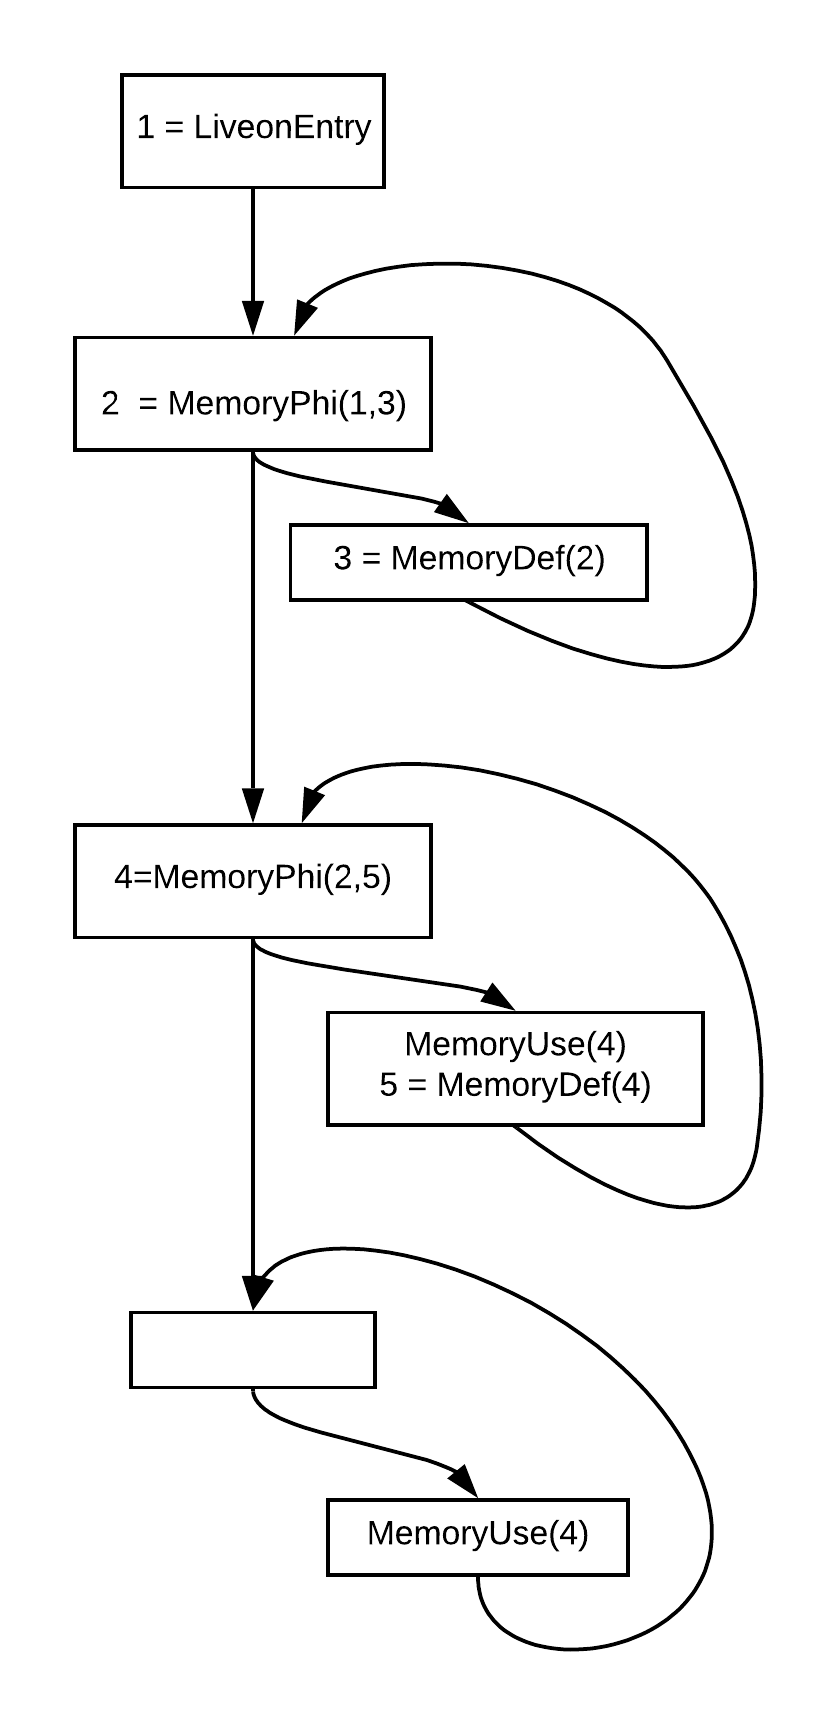
\includegraphics[scale=0.6]{images/memorySSa-impl.png}
\captionof{figure}{Memory SSA of \autoref{memorySSa-impl-code} }
\label{memorySSa-impl}
%         \caption{LLVM Memory SSA Virtual IR}
%         \label{memorySSa-impl}     
%  \begin{figure}
%     \begin{subfigure}{.45\textwidth}
%         \centering
%         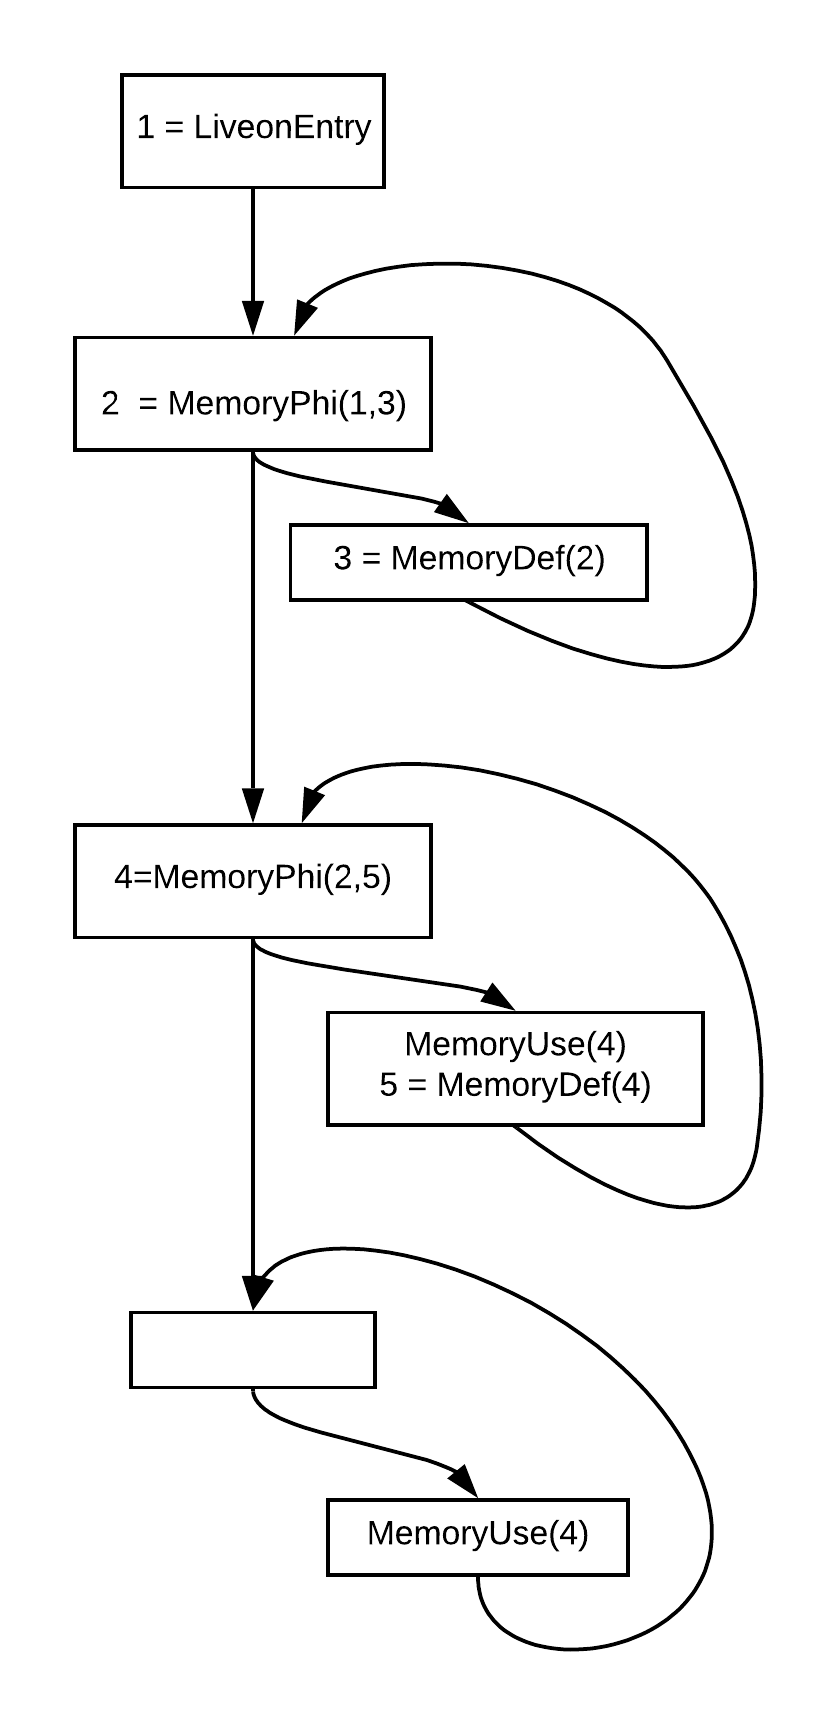
\includegraphics[scale=0.6]{images/memorySSa-impl.png}
%         \caption{LLVM Memory SSA Virtual IR}
%         \label{memorySSa-impl}     
%     \end{subfigure}%
%     \caption{ LLVM MemorySSA Example }
%     \label{LLVMMemorySSA-exmpl}
% %     \vspace{-80pt}
% \end{figure}
\end{minipage}

% \begin{figure}
% %  \hspace*{-10pt}
%     \centering
%     \begin{subfigure}{0.45\textwidth}
%         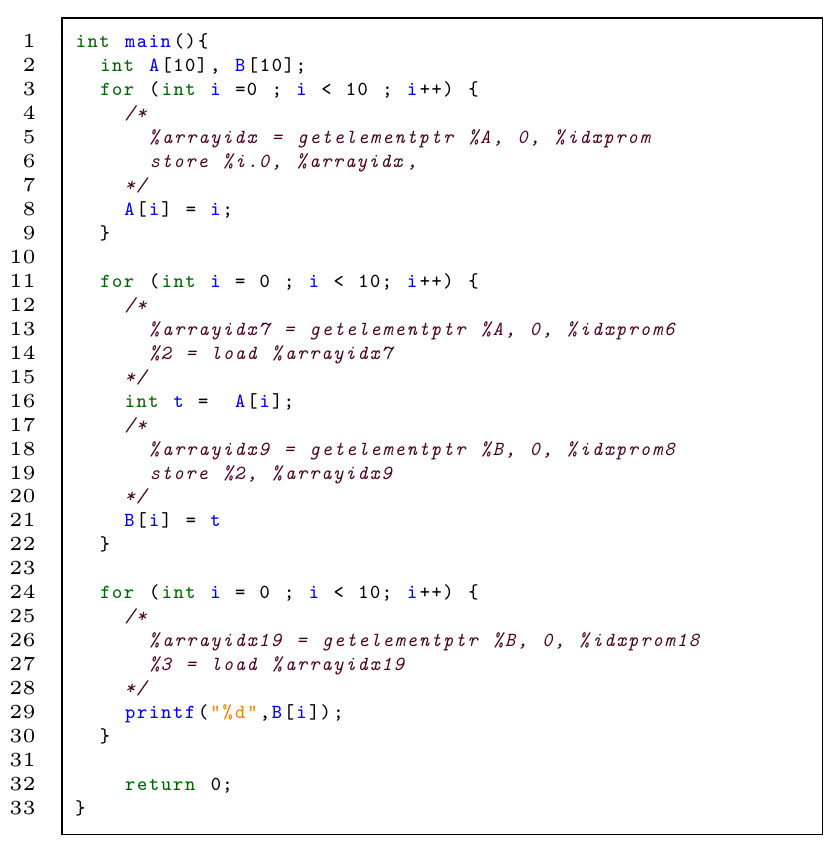
\includegraphics[scale=0.45]{images/memorySSa-impl-code.png}
%         \caption{Code Fragment}
%         \label{memorySSa-impl-code}     
%     \end{subfigure}%    
%     \hspace{40pt}
%     \begin{subfigure}{.45\textwidth}
%         \centering
%         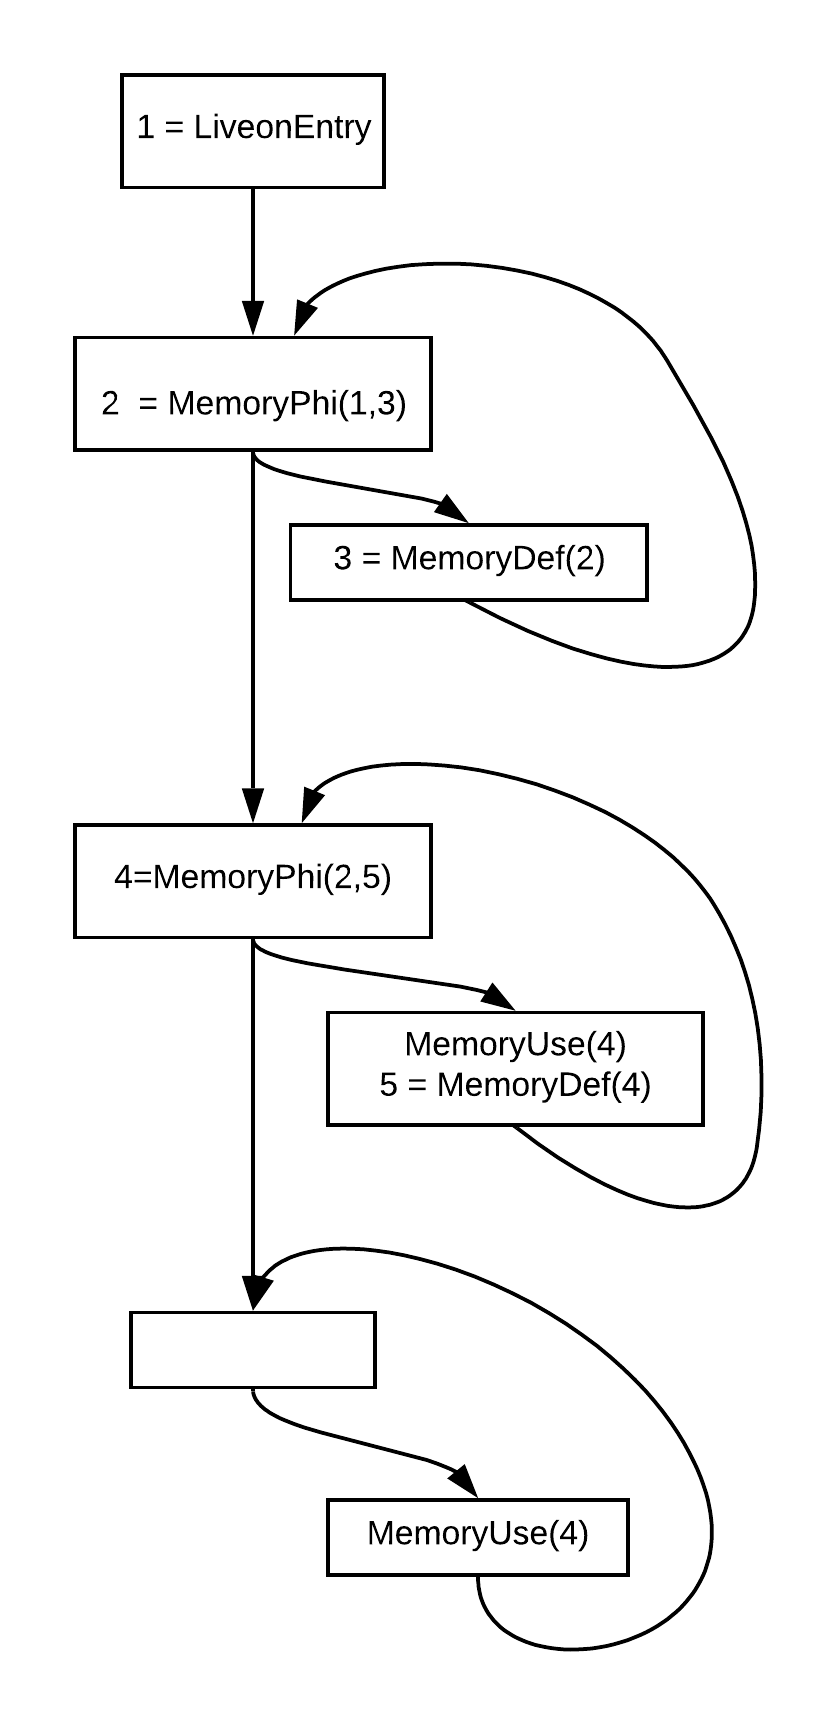
\includegraphics[scale=0.6]{images/memorySSa-impl.png}
%         \caption{LLVM Memory SSA Virtual IR}
%         \label{memorySSa-impl}     
%     \end{subfigure}%
%     \caption{ LLVM MemorySSA Example }
%     \label{LLVMMemorySSA-exmpl}
% %     \vspace{-80pt}
% \end{figure}

Now, we can see the difference between the LLVM memory SSA, 
\autoref{memorySSa-impl} and the array def-use chains  
required for our analysis \autoref{fig:memorySSA-example1}.
We developed a dataflow analysis to 
extract the 
array def-use chains from the LLVM Memory SSA, whenever we can disambiguate the memory variable
that each load/store instruction refers to. 
So, for any store instruction, for example line 22, \autoref{memorySSa-impl-code}, we can analyze the 
LLVM IR, and trace the value that the store instruction refers to, 
which is ``B'' as per the comment in line 19. 
% In this example, line 18, refers to memory variable B, and 
% hence clearly, the $5=MemoryDef(4)$ does not clobber memory variable A. 

We perform an analysis 
on the LLVM IR, which tracks the set of memory variables that each 
LLVM load/store instruction refers to. 
It is a context-sensitive and flow-sensitive 
iterative data flow analysis that associates each MemoryDef/MemoryUse with a set of memory variables. The result of this analysis is an
array SSA form, for each array variable, to tracks its def-use chain, 
similar to the example in \autoref{fig:memorySSA-example1}.
% If the set is a singleton set, then it is a \textit{Must} access, 
% otherwise, it is a \textit{May} access. 
% \begin{minipage}{.45\textwidth}
% \subsection{Validation of data mapping}
% % After the data flow analysis on the memory SSA, we  have the 
% % memory def-use chains. 
% Also, the 
% analysis of \autoref{interpreting-openmp-pragmas} interprets 
% the memory copies introduced by the omp map clauses. Now as explained in 
% section \autoref{s3}, for every pair of Memory def-uses, we 
% verify if the map clause respects that relation. We use the 
% LLVM ''OptimizationRemarkEmitter'' to output the result of our 
% analysis. As we had classified each memory access as must/may, we 
% classify the must violations as Errors, and the may violations as warnings.
% We can prove that the Must violations, found out by our analysis are real bugs in memory mapping 
% clause in the user program.
% \vspace*{-10pt}
\subsubsection{Scalar Evolution Analysis}
LLVM Scalar Evolution is a very powerful technique
that can be used to analyze the change in 
the value of scalar variables over iterations of a loop. 
We can use the SCEV analysis to represent the loop induction variables 
as chain of recurrences. This mathematical representation 
can then be used to analyze the variables used to index into memory 
operations. 
% The SCEV representation in \autoref{memorySSa-impl-code} for variable $i$ on line 16 is `` $\{0,+,1\}<\%for.Line11>$ ''. 
% \begin{itemize}
%  \item The first term of the SCEV is the initial value
%  \item Second term is a mathematical step operation, 
%  in this case it is the increment operator
%  \item Third term is the value which is used to apply the step operation,
%  in this case it is increment by 1,
%  it can also be another SCEV to express chain of recurrences
%  \item SCEV also contains the corresponding enclosing for loops
% \end{itemize}
For our analysis, we need the range of a memory index expression. 
That is the minimum and maximum values, 
of the index expression of any memory address. 
The LLVM SCEV 
analysis can be used to evaluate the maximum value of any variable within 
a loop nest.
to get the maximum number of iterations
of a loop. 
This value can be used to evaluate the maximum value of the SCEV
expression.
We implemented an analysis for array sections, 
that given a load/store, uses the LLVM SCEV analysis, to compute the minimum and maximum values of 
the corresponding index into the memory access. 
% This minimum and maximum can be an expression in terms of program variables. 
% We use this analysis to extract the array sections accessed by any memory load/store. If the SCEV analysis fails to 
% analyze a variable, then we approximate the array section 
% to the maximum size of the array.
% If the memory load/store is from a static array, 
% then the bounds of the array are compile time constants. 
If the analysis fails, then we default to the maximum array size, 
which is either a static array, or can be extracted from the LLVM
memory  \textit{alloc} instructions.
% \vspace{-10pt}
% Otherwise we parse the arguments of the call to memory alloc (malloc), 
% to get the bounds of the corresponding memory variable.
% 
% There are three main cases for the result of SCEV analysis
% \begin{enumerate}
%  \item The upper and lower bounds are compile time constants
%  \item The upper and lower bounds are expressions of program variables
%  \item SCEV is an unknown or cannot be evaluated
% \end{enumerate}
% 
% For our analysis, we approximate the case 2 and 3, with the maximum 
% size of an array. If the memory load/store is from a static array, 
% then the bounds of the array are compile time constants. 
% Otherwise we parse the arguments of the call to memory alloc (malloc), 
% to get the bounds of the corresponding memory variable.
% 
% So, the Array Sections analysis works only if the range of a 
% memory access can be evaluated to compile time integer constants. 
% 
% Finally we use the algorithm from \autoref{dataMapAnalysisAlgo} to warn 
% the user if incorrect array sections are used in the memory map clause.
% The warning can be of the following types
% \begin{itemize}
%  \item Array section accessed on the device environment is larger than the array section mapped onto the device, that is out of bounds access on the device
%  \item Array section mapped out of the device environment to the host, is smaller/subset of what the host environment accesses. 
% \end{itemize}
% __tgt_target_data_begin,3.c:16,3.c:16,0,persistentIn,copyin,A[0:5],persistentOut,copyout,alloc,B[0:10],                                                                                                            
% __tgt_target,3.c:17,3.c:21,0,persistentIn,A[0:10],B[0:10],copyin,persistentOut,copyout,A[0:10],B[0:10],alloc,


\section{Evaluation and Case Studies}
\label{s5}
% 
% \begin{minipage}{.45\textwidth}
% \begin{lstlisting}[style=customcnonum, frame=tlrb, caption={DRACC File 22}, label=eval-f22]
%  15 int init(){
%  16     for(int i=0; i<C; i++){
%  17         for(int j=0; j<C; j++){
%  18             b[j+i*C]=1;
%  19         }
%  20         a[i]=1;
%  21         c[i]=0;
%  22     }
%  23         return 0;
%  24 }
%  25                                                                                                                                                                                                                
%  26 
%  27 int Mult(){
%  28 
%  29     #pragma omp target map(to:a[0:C]) map(tofrom:c[0:C]) map(alloc:b[0:C*C]) device(0)
%  30     {
%  31         #pragma omp teams 
%                     distribute parallel for
%  32         for(int i=0; i<C; i++){
%  33             for(int j=0; j<C; j++){
%  34                 c[i]+=b[j+i*C]*a[j];
% 
% \end{lstlisting}
% \end{minipage} \hfill 
% \begin{minipage}{.45\textwidth}
% \begin{lstlisting}[style=customcnonum, frame=tlrb, caption={DRACC File 26}, label=eval-f26]
%  29     #pragma omp target 
%                 enter data map(to:a[0:C],b[0:C*C],c[0:C]) device(0)
%  30     #pragma omp target device(0)
%  31     {
%  32         #pragma omp teams 
%                         distribute parallel for
%  33         for(int i=0; i<C; i++){
%  34             for(int j=0; j<C; j++){
%  35                 c[i]+=b[j+i*C]*a[j];
%  36             }
%  37         }
%  38     }        
%  39     #pragma omp target exit
%                 data map(release:c[0:C]) 
%                 map(release:a[0:C],b[0:C*C]) device(0)
%  40     return 0;
%  41 }
%  42 
%  43 int check(){
%  44     bool test = false;
%  45     for(int i=0; i<C; i++){
%  46         if(c[i]!=C){
% 
% \end{lstlisting}
% \end{minipage}
%  
%  
%  \begin{minipage}{.45\textwidth}
% \begin{lstlisting}[style=customcnonum, frame=tlrb, caption={DRACC File 23}, label=eval-f23]
% 28 int Mult(){
%  29     
%  30     #pragma omp target map(to:a[0:C],b[0:C]) map(tofrom:c[0:C]) device(0)
%  31     {
%  32         #pragma omp teams 
%                         distribute parallel for
%  33         for(int i=0; i<C; i++){
%  34             for(int j=0; j<C; j++){
%  35                 c[i]+=b[j+i*C]*a[j];
%  36             }
%  37         }
%  38     }  
% \end{lstlisting}
% \end{minipage}\hfill 
% \begin{minipage}{.45\textwidth}
% \begin{lstlisting}[style=customcnonum, frame=tlrb, caption={DRACC File 30}, label=eval-f30]
% 19 int init(){
%  20     for(int i=0; i<C; i++){
%  21         for(int j=0; j<C; j++){
%  22             b[j+i*C]=1;
%  23         }
%  24         a[i]=1;
%  25         c[i]=0;                                                                                      
%  26     }
%  ~ 
%  31 int Mult(){
%  32     
%  33     #pragma omp target 
%             map(to:a[0:C],b[0:C*C]) map(from:c[0:C*C]) device(0)
%  34     {
%  35         #pragma omp teams 
%                         distribute parallel for
%  36         for(int i=0; i<C; i++){
%  37             for(int j=0; j<C; j++){
%  38                 c[i]+=b[j+i*C]*a[j];
% \end{lstlisting}
% \end{minipage} 
\
For evaluating OMPSan we use the DRACC\cite{dracc-benchmark} suite, which is a 
benchmarks for data race detection on accelerators, and
also includes several data mapping errors also.
% from Aachen University 
%to evaluate our tool. 
\autoref{dracc-errors} shows some distinct errors found 
by our tool in the benchmark\cite{dracc-benchmark} and the examples of
\autoref{s2}. We were able to find the 15 known 
data mapping errors in the DRACC benchmark. 
% The last 3 rows of the table shows the errors pointed out by our 
% tool, for the examples from the motivation section. 
% \vspace{-20pt}
% For example in file number 22,\autoref{eval-f22} the map clause on 
% line 29 is using the \textit{alloc} attribute while line 34 is 
% actually reading the array b, that was defined on line 18, so 
% our tool points out the error message that the ``to'' clause is mssing.
% For \autoref{eval-f26} ``c'' is updated on the device at line 34, 
% but it is not mapped back, and our error points out that the 
% ``from/update'' clause is missing.
% For \autoref{eval-f30}, ``c'' is initialized on line 25, 
% but the host variable is not mapped to the device, 
% when creating the device environment at line 33. 
% For \autoref{eval-f23}, only ``C'' elements of ``b''
% are mapped to the device, while the actual size of ``b'' 
% is ``C*C''. Our tool is able to track the malloc call 
% to flag this usage as a warning.
% \vspace{-10pt}
\begin{table}
    \caption{Errors found in the DRACC Benchmark and other examples}
    \label{dracc-errors}
    \begin{center}
        \scriptsize
        \begin{tabular}{ |m{1.5in} | m{3in} |}
            \hline
           File Name & Error/Warning \\ \hline    
           DRACC File 22  & ERROR Definition of :b on Line:18 is not reachable to Line:34, Missing Clause:to:Line:32 \\ \hline    
%            DRACC File 24 & ERROR Definition of :b on Line:18 is not reachable to Line:34 Missing Clause:to:Line:32 \\ \hline 
           DRACC File 26 & ERROR Definition of :c on Line:35 is not reachable to Line:46 Missing Clause:from/update:Line:44 \\ \hline 
           DRACC File 30 & ERROR Definition of :c on Line:25 is not reachable to Line:38 Missing Clause:to:Line:36 \\ \hline 
           DRACC File 23 & WARNING Line:30 maps partial data of :b smaller than its total size   \\ \hline 
           Example in \autoref{incorrectegs1} & 
           ERROR Definition of :sum on Line:5 is not 
           reachable to Line:6 Missing Clause:from/update:Line:6 \\ \hline  
%            Example in \autoref{incorrectegs3} & 
%            ERROR Definition of :B on Line:8 is not
%            reachable to Line:12 Missing Clause:from/update:Line:10 
%            \\ \hline 
           Example in \autoref{incorrectegs2} &
           ERROR Definition of :A on Line:7 is not 
           reachable to Line:9 Missing Clause:from/update:8
           \\ \hline                              
        \end{tabular}        
    \end{center}
\end{table} 
\vspace{-20pt}
% \begin{table}
%     \caption{Errors found in the DRACC Benchmark}
%     \label{dracc-errors}
%     \begin{center}
%         \scriptsize
%         \begin{tabular}{ |m{1.5in} | m{3in} |}
%             \hline
%            File Name & Error/Warning \\ \hline    
%            DRACC File 22 \autoref{eval-f22} & ERROR Definition of :b on Line:18 is not reachable to Line:34, Missing Clause:to:Line:32 \\ \hline    
% %            DRACC File 24 & ERROR Definition of :b on Line:18 is not reachable to Line:34 Missing Clause:to:Line:32 \\ \hline 
%            DRACC File 26 \autoref{eval-f26}& ERROR Definition of :c on Line:35 is not reachable to Line:46 Missing Clause:from/update:Line:44 \\ \hline 
%            DRACC File 30 \autoref{eval-f30}& ERROR Definition of :c on Line:25 is not reachable to Line:38 Missing Clause:to:Line:36 \\ \hline 
%            DRACC File 23 \autoref{eval-f23}& WARNING Line:30 maps partial data of :b smaller than its total size   \\ \hline 
%            Motivation Ex \autoref{incorrectegs1} & 
%            ERROR Definition of :sum on Line:5 is not 
%            reachable to Line:6 Missing Clause:from/update:Line:6 \\ \hline  
%            Motivation Ex \autoref{incorrectegs3} & 
%            ERROR Definition of :B on Line:8 is not
%            reachable to Line:12 Missing Clause:from/update:Line:10 
%            \\ \hline 
%            Motivation Ex \autoref{incorrectegs2} &
%            ERROR Definition of :A on Line:7 is not 
%            reachable to Line:9 Missing Clause:from/update:8
%            \\ \hline 
%            \hline                          
%         \end{tabular}        
%     \end{center}
% \end{table}
% The errors were explained in \autoref{s2}
\subsection{Analysis Time}
We also measured the runtime of the analysis, 
\autoref{runtime} shows the time to run OMPSan, on few SPEC ACCEL and 
NAS parallel benchmarks. 
% We compare it with the time to compile the programs with ``-O3'' flag. 
Due to the context and flow sensitive data flow analysis implemented in 
OMPSan, 
its analysis time can be significant; 
however the analysis time is less than or equal to the \textit{-O3}
compilation time in all cases.
%its runtime is significant, and almost as much as the 
%time to compile the entire program with ``-O3''. 
\begin{table} 
\vspace{-20pt}
    \caption{Time to Run OMPSan}
    \label{runtime}
    \begin{center}
        \scriptsize
        \begin{tabular}{ | c | c | c |}
            \hline
           Benchmark Name &  -O3 Compilation Time (sec)
           & OMPSan Runtime (sec) \\ \hline    
           SPEC 504.polbm & 17 & 16 \\ \hline    
           SPEC 503.postencil & 3 & 3 \\ \hline    
           SPEC 552.pep  & 7 & 4 \\ \hline    
           SPEC 554.pcg & 15 & 9\\ \hline    
           NAS FT & 32 & 15 \\ \hline    
           NAS MG & 34 & 31              \\ \hline                       
        \end{tabular}        
    \end{center}
\end{table}\vspace{-40pt}
\subsection{Diagnostic Information}
\label{diagnostic}
Another major use case for OMPSan, is to help OpenMP developers 
understand 
the data mapping behavior of their source code. 
For example, \autoref{nas-ft-1} shows a code fragment 
from the benchmark ``FT'' in the ``NAS'' suite.
% We argue that it is very difficult to read 
% this openmp target code, as line 311 explicitly 
% maps every array variable with the ``alloc'' 
% map type. Since, these are global variables, the 
% semantics of this \texttt{target map} depend 
% on the previous occurrences of the mapping clause. 
Our tool can generate the following information
diagnostic information on the current version 
 of the data mapping clause.
\begin{itemize}
    \vspace{-4pt}
 \item \texttt{$\_\_tgt\_target\_teams$}, from::``ft.c:311'' to ``ft.c:331''
 \item Alloc: $u0\_imag[0:8421376],u0\_real[0:8421376]$
 \item Persistent In :: $twiddle[0:8421376]$, 
 $u1\_imag[0:8421376],u1\_real[0:8421376]$
 \item  Persistent Out ::  $twiddle[0:8421376],u0\_imag[0:8421376],u0\_real[0:8421376],u1\_imag[0:8421376],u1\_real[0:8421376]$
 \item Copy In:: \textit{Null}, Copy Out:: \textit{Null} 
\end{itemize}
% Similarly, the data mapping for the function $cffts3\_pos$ \autoref{nas-ft-2}, is as shown below,
% \begin{itemize}
%     \vspace{-4pt}
%  \item \texttt{$\_\_tgt\_target\_teams$}, from::``ft.c:1180'' to ``ft.c:1276''
%  \item Persistent In ::
%  $gty1\_imag[0:16777216],gty1\_real[0:16777216],gty2\_imag[0:16777216],gty2\_real[0:16777216],logd3[0:0],u0\_imag[0:8421376],u0\_real[0:8421376],u1\_imag[0:8421376],u1\_real[0:8421376],u\_imag[0:257],u\_real[0:257]$
%  \item Persistent Out: $u1\_imag[0:8421376],u1\_real[0:8421376],u\_imag[0:257],u\_real[0:257]$
%  \item Copy Out: $gty1\_imag[0:16777216],gty1\_real[0:16777216],gty2\_imag[0:16777216],gty2\_real[0:16777216],u0\_imag[0:8421376],u0\_real[0:8421376]$
% \end{itemize}
\hspace{-10pt}
\begin{minipage}{1.1\textwidth}
\begin{lstlisting}[style=customcnonum,basicstyle=\scriptsize, frame=tlrb, caption={\textit{evolve} from NAS/ft.c}, label=nas-ft-1]
 307 static void evolve(int d1, int d2, int d3)
 308 {
 309  int i, j, k;
 311 #pragma omp target map (alloc: u0_real,u0_imag,u1_real,u1_imag,twiddle)
 312  {
 313 #pragma omp teams distribute
 314   for (k = 0; k < d3; k++) {
 315 #pragma omp parallel for
 316    for (j = 0; j < d2; j++) {
 317 #pragma omp simd
 318     for (i = 0; i < d1; i++) {
 319      u0_real[ ... ] = u0_real[ ... ]*twiddle[ ... ];
 321      u0_imag[ ... ] = u0_imag[ ... ]*twiddle[ ... ];
\end{lstlisting}
\end{minipage}  
% \hfill 
% \begin{minipage}{.45\textwidth}
% \begin{lstlisting}[style=customcnonum, frame=tlrb, caption={\textit{cffts3\_pos} from NAS/ft.c}, label=nas-ft-2]
%  1153 static void cffts3_pos(int is, int d1, int d2, int d3)
% 1154 {
% 1155   int logd3;
% 1156   int i, j, k, ii;
% 1157   int l, j1, i1, k1;
% 1158   int n1, li, lj, lk, ku, i11, i12, i21, i22;
% 1159   double uu1_real, x11_real, x21_real;
% 1160   double uu1_imag, x11_imag, x21_imag;
% 1161   double uu2_real, x12_real, x22_real;
% 1162   double uu2_imag, x12_imag, x22_imag;
% 1163   double temp_real, temp2_real;
% 1164   double temp_imag, temp2_imag;
% 1165 
% 1166   logd3 = ilog2(d3);
% ~
% 1180 #pragma omp target teams distribute collapse(2)
% 1181     for (j = 0; j < d2; j++) {
% 1182 //#pragma acc loop vector independent
% 1183 //#pragma omp simd
% 1184       for (i = 0; i < d1; i ++) {
% 1185 #pragma omp parallel for
% 1186         for (k = 0; k < d3; k++) {
% 1187           gty1_real[j][k][i] = u1_real[k*d2*(d1+1) + j*(d1+1) + i];
% 1188           gty1_imag[j][k][i] = u1_imag[k*d2*(d1+1) + j*(d1+1) + i];
% 1189         }
% 1190 
% 
% \end{lstlisting}
% \end{minipage} 
\vspace{-10pt}
\subsection{Limitations}
\label{limitation}
Since OMPSan is a static analysis tool, 
it includes a few limitations. OMPSan, 
% as listed below: 
\vspace{-2pt}
\begin{itemize}
 \item Supports statically and dynamically allocated array variables, 
 but cannot 
 handle dynamic data structures like linked lists
%  (Future extension, use shape analysis)
 It can possibly be 
 addressed in future through advanced static analysis techniques (like shape analysis).
 \item Cannot handle target regions inside recursive functions. 
%  It can 
%  be addressed by improving our context 
%  sensitive analysis.
 It can possibly be addressed in future work by improving our context 
 sensitive analysis.
 \item Can only handle compile time 
 constant array sections, and constant loop bounds.
%   it requires support to 
%  compare the equivalence of two symbolic expressions.
%  OMPSan can be extended in the future
 We can handle runtime expressions, by adding static analysis support to 
 compare the equivalence of two symbolic expressions.
 \item Cannot handle “declare target” 
 since it requires analysis across LLVM modules.
 \item May report false positives for irregular array accesses.
  For example, even if only a small section of the array is updated, 
  our analysis may assume the entire array was updated. More 
  expensive analysis like symbolic analysis can be used to 
  improve the precision of the static analysis.
  \item May fail if Clang/LLVM introduces bugs while 
  lowering OpenMP pragmas to the RTL calls in the LLVM IR.
  Since, 
  we rely heavily on static analysis like Memory SSA and SCEV analysis, 
  it is difficult to implement our algorithm on the clang AST.
  \item May report false positives, if the OpenMP program relies 
  on some dynamic reference count mechanism. 
  That is our algorithm may not be able to 
  statically track a variable's reference count, at the data map clause, 
  and the diagnostics will be inaccurate. Runtime debugging approach 
  will be required to handle such cases.
  
%  since it is 
%  moved to a different module in LLVM IR. 
%  since in LLVM IR, 
%  the ``declare'' region is moved to a separate region, this 
%  can also be fixed if we can analyze the modules together. 
\end{itemize}
% 
% Our analysis shows the following error for \autoref{eval-ex1}, 
% that was used as motivation in \autoref{s2},
% \begin{verbatim}
% ERROR Definition of :sum on Line:5 is not 
% reachable to Line:6 Missing Clause:from/update:Line:6 
% \end{verbatim}
% Since the user missed the explicit map clause for ``sum'', 
% the default mapping was first private, and the value was not mapped back to the host, hence line 6 used a stale version of the variable sum.
% % \autoref{data-mapping-example} shows the memory copies deduced by our tool.
% 
% As explained in motivation \autoref{s2}, for \autoref{eval-ex2} our tool is able to catch the data mapping issue, but please note that
% the Openmp 5.0 spec has been modified so that this is no longer 
% a bug according to OpenMP 5.0.
% \begin{verbatim}
%  ERROR Definition of :B on Line:8 is not
%  reachable to Line:12 Missing Clause:from/update:Line:10
% \end{verbatim}
% 
% Our tool is also able to catch the error for \autoref{incorrectegs2}, 
% from \autoref{s2}.
% \begin{verbatim}
% ERROR Definition of :A on Line:7 is not 
% reachable to Line:9 Missing Clause:from/update:8
% \end{verbatim}
% The reason for this error was that, the reference 
% count for variable A is incremented at line 5, 
% after it was set to 1 at line 3,
% and device-host memory copy is inserted only if the reference count 
% is decremented to zero.
% % \autoref{data-mapping-example} shows the reason for this error, A 
% % is not copied out at line 7, hence the read on line 9 was stale. 
% 
% \begin{minipage}{.4\textwidth}
% \begin{lstlisting}[style=customc, frame=tlrb, caption={Wrong Usage of default map on Reduction Scalar}, label=eval-ex1]
% int A[N], sum=0, i;
% #pragma omp target
% #pragma omp teams distribute parallel for reduction(+:sum)
%   for(i=0; i<N; i++) 
%     sum += A[i];
%   printf("\n%d",sum);
% \end{lstlisting}
% \end{minipage}\hfill 
% \begin{minipage}{.4\textwidth}
% \begin{lstlisting}[style=customc, frame=tlrb, caption={Usage of alloc vs from}, label=eval-ex2]
% int A[10], B[10];
% for (int i =0 ; i < 10 ; i++)
%     A[i] = i;
% 
% #pragma omp target enter data map(to:A[0:10]) map(alloc:B[0:10])
% #pragma omp target map(alloc:B[0:10])
% for (int i = 0 ; i < 10; i++)
%     B[i] = A[i];
% #pragma omp target exit data map(from:B[0:10])
% 
% for (int i = 0 ; i < 10; i++)
%     printf("%d",B[i]);
% \end{lstlisting}
% \end{minipage} 
% 
% 
%  


% \begin{table}
%     \caption{Compile Time for our Tool}
%     \label{dracc-errors}
%     \begin{center}
%         \scriptsize
%         \begin{tabular}{ |m{0.7in} | m{0.6in} | m{0.7in} |}
%             \hline
%            Benchmark Name & Analysis Runtime (sec) & 
%            Standard Compile Time (sec) \\ \hline    
%            spec accel, 504 polbm & ~16.3 & ~0.15 \\ \hline    
% 
%             \hline               
%            \hline                          
%         \end{tabular}        
%     \end{center}
% \end{table}

% 
% \begin{minipage}{.45\textwidth}
% \begin{lstlisting}[style=customc, frame=tlrb, caption={explicit map}, label=eval-ex2]
% int A[N], sum=0, i;
% #pragma omp target map(tofrom:sum)
% #pragma omp teams distribute parallel for reduction(+:sum)
%   for(i=0; i<N; i++) 
%     sum += A[i];
%   printf("\n%d",sum);
% \end{lstlisting}
% \end{minipage}
% \begin{minipage}{.4\textwidth}
% \begin{lstlisting}[style=customc, frame=tlrb,  caption={Reference Count}, label=eval-ex3]
% define N 100                                                                                            
% int A[N], sum=0;
% #pragma omp target data map(from:A[0:N]) 
%   {
%     #pragma omp target map(from:A[0:N])
%     for(int i=0; i<N; i++) 
%       A[i]=i;
%     for(int i=0; i<N; i++) 
%       sum += A[i];
%   }
% \end{lstlisting}
% \end{minipage}\hfil
% \begin{minipage}{.4\textwidth}
% \begin{lstlisting}[style=customc, frame=tlrb, caption={Update Clause}, label=eval-ex4]
% define N 100                                                                                            
% int A[N], sum=0;
% #pragma omp target data map(from:A[0:N]) 
%   {
%     #pragma omp target map(from:A[0:N])
%     for(int i=0; i<N; i++) 
%       A[i]=i;
%     #pragma omp target update from(A[0:N])  
%     for(int i=0; i<N; i++) 
%       sum += A[i];
%   }
% \end{lstlisting}
% \end{minipage}
% \begin{table}
%     \caption{Output Data mapping }
%     \scriptsize
%     \label{data-mapping-example}
%     \begin{center}
% %         \footnotesize
%         \begin{tabular}{|c |c | m{0.5in} | m{0.4in} | m{0.5in} | m{0.6in} 
%                 | m{0.5in} | m{0.6in} | m{0.5in} |}
%             \hline
%            Listing Name & RTL name & Region Line Begin & 
%            Region Line end & Copy In & Persistent In 
%            & Copy Out & Persistent out & Alloc \\ \hline    
%            \autoref{eval-ex1} & $\_\_tgt\_target\_teams$  
%            & 2 & 5 & A[0:100], sum & & A[0:100]& sum & \\ \hline
%            \autoref{eval-ex2} & $\_\_tgt\_target\_teams$  
%            & 2 & 5 & A[0:100], sum & & A[0:100], sum& & \\ \hline
%            \autoref{eval-ex3} & $\_\_tgt\_data\_begin$  
%            & 3 & 10 &  & & A[0:100] & &A[0:100]  \\ \hline
%            \autoref{eval-ex3} & $\_\_tgt\_target$  
%            & 5 & 7 &  & A[0:100] & &A[0:100] & \\ \hline
%            \autoref{eval-ex4} & $\_\_tgt\_data\_begin$  
%            & 3 & 10 &  & & A[0:100] & &A[0:100]  \\ \hline
%            \autoref{eval-ex4} & $\_\_tgt\_target$  
%            & 5 & 7 &  & A[0:100] & &A[0:100] & \\ \hline
%            \autoref{eval-ex4} & $\_\_tgt\_target\_data\_update$  
%            & 9 & 9 &  & & A[0:100] & & \\ \hline
%            
% %            $\_\_tgt\_target$  
% %            & 7 & 10 &  & A[0:10], B[0:10] & A[0:10] & B[0:10] & \\ \hline               
% %            $\_\_tgt\_target\_data\_end$  
% %            & 10 & 10 &  & & B[0:10] & & \\ \hline               
%            \hline                          
%         \end{tabular}        
%     \end{center}
% \end{table}


\section{Related Work and Conclusion}
\vspace*{-5pt}
Managing data transfers to and from GPUs has always been 
an important problem for GPU programming. 
Several solutions have been proposed to help 
the programmer in managing the data movement.
CGCM \cite{Jablin:2011:ACC:1993316.1993516} was one of the first
systems with static analysis to manage CPU-GPU communications. 
It was followed by \cite{Jablin:2012:DMD:2259016.2259038}, a 
dynamic tool for automatic   
CPU-GPU data management. 
The OpenMPC compiler \cite{Lee:2010:OEO:1884643.1884674} also 
proposed a static analysis to insert data transfers automatically.
\cite{6877281} proposed a directive based approach for specifying CPU-GPU memory transfers, which included compile-time/runtime methods to verify the correctness of the directives and also identified opportunities for performance optimization.
\cite{Pai:2012:FEA:2370816.2370824} proposed a compiler analysis to 
detect potential stale accesses and uses a runtime to initiate transfers as necessary, for the X10 compiler. \cite{Thangamani:2018:ORD:3243176.3243209} 
also proposed a static analysis technique to optimize 
the data transfers for the X10.
\cite{Mendonca:2017:DAA:3086564.3084540} has also worked on automatically 
inferring the OpenMP mapping clauses using some static analysis. 

% There have been several work for debugging and correctness tools for OpenMP 
% programming, \cite{reissmann2018diagnosing}, \cite{drebes2016language}, \cite{protze2015lessons}.

In this paper, we have developed OMPSan, a static analysis 
tool to interpret the semantics of the OpenMP map clause, 
and deduce the data transfers introduced by the clause. 
Our algorithm tracks the reference count for individual variables 
to infer the effect of the data mapping clause on the host and device data 
environment.  
We have developed a data flow analysis, on top of LLVM memory 
SSA to capture the def-use information of Array variables. 
We use LLVM Scalar Evolution, to improve the precision of 
our analysis by estimating the range of locations accessed 
by a memory access. This enables the OMPSan to handle array sections also. 
Then OMPSan computes how the data mapping clauses modify 
the def-use chains of the baseline program, and use 
this information to 
validate if the data mapping in the OpenMP program respects the 
original def-use chains of the baseline sequential program. 
Finally OMPSan reports diagnostics, to help 
the developer debug and understand the usage of \texttt{map}
clauses of their program. 
We believe the analysis presented in this paper is very powerful and 
can be developed further for data mapping optimizations also.
We also plan to combine our static analysis 
with a dynamic debugging tool, that would enhance the performance 
of the dynamic tool and also address the limitations of the static analysis.
% Then our analysis validates how the def-use chains 
% of the baseline program are modified by the data mapping, 
% and reports if it is not as expected.

\bibliographystyle{splncs04}
% \footnotesize
% \setlength{\bibsep}{3pt}
\bibliography{acmbib}

\end{document}
